\section{Discrete Sensitivity Analysis}
% -.-.-.-.-.-.-.-.-.-.-.-.-.-.-.-.-.-.-.-.-.-.-.-.-.-.-.-.-.-.-.-.-.-.-
\subsection{Formulation}
The derivation of the discrete sensitivity equations starts with the discrete form of the governing equations. For the linear case, the governing equation \eqref{eq:C2_generalGoverningEquation} is discretized as shown in Equation \eqref{eq:C2_discreteGoverningEquation}
%
\begin{equation}\label{eq:C2_discreteGoverningEquation}
    \left[ K \right] \left[ U \right] = \left[ F \right]
\end{equation}
%
Where $[K]$ is the discrete operator that represents the governing equation; $[U]$ is the vector of the response variables defined at each of the degrees of freedom, and $[F]$ is the vector of the applied loads. The sensitivity of this system to design variable $b$ is derived by differentiating Equation \eqref{eq:C2_discreteGoverningEquation}.
%
\begin{equation}\label{eq:C2_discreteSensitivityEquation}
    \left[ K \right] \left[ \frac{\partial U}{\partial b} \right] = 
    \left[ \frac{\partial F}{\partial b} \right] - 
    \left[ \frac{\partial K}{\partial b} \right] \left[ U \right]
\end{equation}
%
Solving Equation \eqref{eq:C2_discreteSensitivityEquation} yields a solution for sensitivity of response variable, $\partial U/\partial b$. This is achievable if the values of $\partial F/\partial b$ and $\partial K/\partial b$ are known. It should be noted that $U$ is calculated by solving the governing equation \eqref{eq:C2_discreteGoverningEquation}. For the case of design independent loads, $\partial F/\partial b$ is equal to zero; this happens in many situations such as design optimization with pure mechanical loads. This assumption is violated for the cases when changing the design variables alter the loadings on the structure. The best example for this case is the design of thermally loaded structures where, due to thermal expansions, changing the size of elements will affect the thermal loadings \cite{deaton2013stiffening}. Calculating the $\partial K/\partial b$ term requires a detailed understanding of the discretization approach. This often requires source code modification that makes this method difficult to implement for commercial codes such as ABAQUS or FLUENT. The discrete method is an accurate approach for calculating the sensitivities as will be demonstrated with the following examples; however, it is almost impossible to implement in general-purpose solvers due to non-accessibility of the source code. The discrete sensitivity analysis is build into a couple of analysis tools such as Nastran, ASTROS, and OptiStruct and can be used for sensitivity analysis.
% -.-.-.-.-.-.-.-.-.-.-.-.-.-.-.-.-.-.-.-.-.-.-.-.-.-.-.-.-.-.-.-.-.-.-.-.-.-.-.-.-.-.-.-.-.-
\subsection{Implementation on heat transfer problem}
The discrete sensitivity equations are formulated by discretizing the governing equation \eqref{eq:C2_laplaceEquation} using the finite difference method. It should be noted that finite difference is used for discretization of the continuum governing equation and not for the sensitivity calculation. Other techniques, such as finite volume or finite elements, can be used for the discretization of the governing equations as well. For this problem, the design variable affects the shape of the domain which is related to the distance between the nodes in a discrete manner. Therefore, for the sake of sensitivity analysis, it is required to keep the nodal distances in the discretized solution as well. The domain is discretized by using six nodes as shown in Figure \ref{fig:C2_discretizedDomain}.
%
\begin{figure}[h]
    \centering
    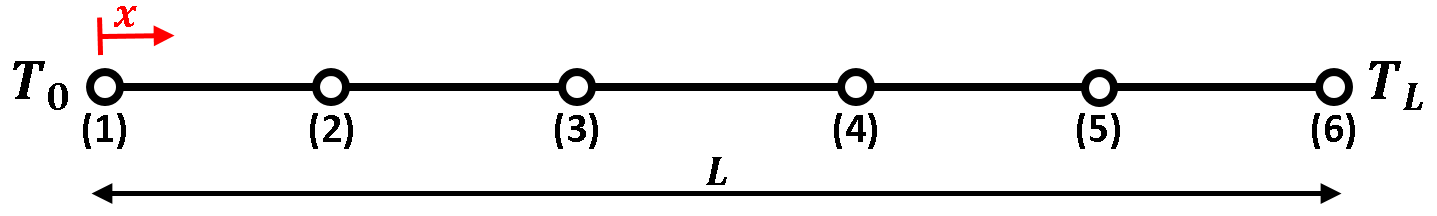
\includegraphics[width=14.00cm]{Chapter_2/figure/benchmark_case_computational_domain.png}
    \caption{One dimensional computational domain for the heat conduction problem.}
    \label{fig:C2_discretizedDomain}
\end{figure}
%
The second derivative of Equation \eqref{eq:C2_laplaceEquation} needs to be approximated for discretization. This is done by writing the Taylor series expansion of temperature at an arbitrary location $x_i$. By using the central difference method, the second order approximation for the second order derivative is written as shown in Equation \eqref{eq:C2_finiteDifferenceSchemes}.

To maintain the generality, we assume that distance of node $T_i$ to $T_{i+1}$ is $\Delta_i$ and the distance of node $T_i$ to $T_{i-1}$ is $\Delta_{i-1}$.
%
\begin{equation}\label{eq:C2_finiteDifferenceSchemes}
    \frac{\partial^2 T}{\partial x^2} = 
    \frac{T_{i-1} \Delta_{iL} - 
          T_{i} (\Delta_{iL} + \Delta_{iR}) + 
          T_{i+1} \Delta_{iR}}
         {\dfrac{1}{2} \left[ \Delta_{iL} \Delta_{iR}^2 + 
                             \Delta_{iL}^2 \Delta_{iR} \right]}
\end{equation}
%
The discretized governing equation of \eqref{eq:C2_finiteDifferenceSchemes} is written in a matrix form as shown in Equation \eqref{eq:C2_laplaceEquationMatrixForm}.
%
\begin{equation}\label{eq:C2_laplaceEquationMatrixForm}
    \begin{bmatrix}
        \frac{-2}{\Delta_{1} \Delta_{2}} &
        \frac{2}{\Delta_{1} \Delta_{2} + \Delta_{1}^2} &
        0 &
        0 &
        \\
        \frac{2}{\Delta_{3}^2 + \Delta_{2} \Delta_{3}} & 
        \frac{-2}{\Delta_{2} \Delta_{3}} &
        \frac{2}{\Delta_{2} \Delta_{3} + \Delta_{2}^2} &
        0
        \\
        0 &
        \frac{2}{\Delta_{4}^2 + \Delta_{3} \Delta_{4}} & 
        \frac{-2}{\Delta_{3} \Delta_{4}} &
        \frac{2}{\Delta_{3} \Delta_{4} + \Delta_{3}^2} &
        \\
        0 &
        0 &
        \frac{2}{\Delta_{5}^2 + \Delta_{4} \Delta_{5}} & 
        \frac{-2}{\Delta_{4} \Delta_{5}}
    \end{bmatrix}
    \begin{bmatrix}
        T_2 \\
        T_3 \\
        T_4 \\
        T_5
    \end{bmatrix}
    =
    -\begin{bmatrix}
         \frac{2T_1}{\Delta_{2}^2 + \Delta_{1} \Delta_{2}} \\
         0 \\
        0 \\
        \frac{2T_6}{\Delta_{5} \Delta_{4} + \Delta_{5}^2}
    \end{bmatrix}
\end{equation}
%
To verify the discretization process, we compare the analytical solution of this problem with the result of Equation \eqref{eq:C2_laplaceEquationMatrixForm} in Figure \ref{fig:C2_verificationOfSolver}. For this problem we choose $T_1 = 0$, $T_6 = 1$ as the boundary conditions and $L = 1$.  As shown in this figure, the discrete and continuum results match very well for a different number of nodes. This is done by comparing the absolute maximum error between the analytical and approximate results as shown in Table \ref{table:C2_solutionError}.
%
\begin{figure}[H]
    \centering
    \subfigure[$n = 6$]
    {
    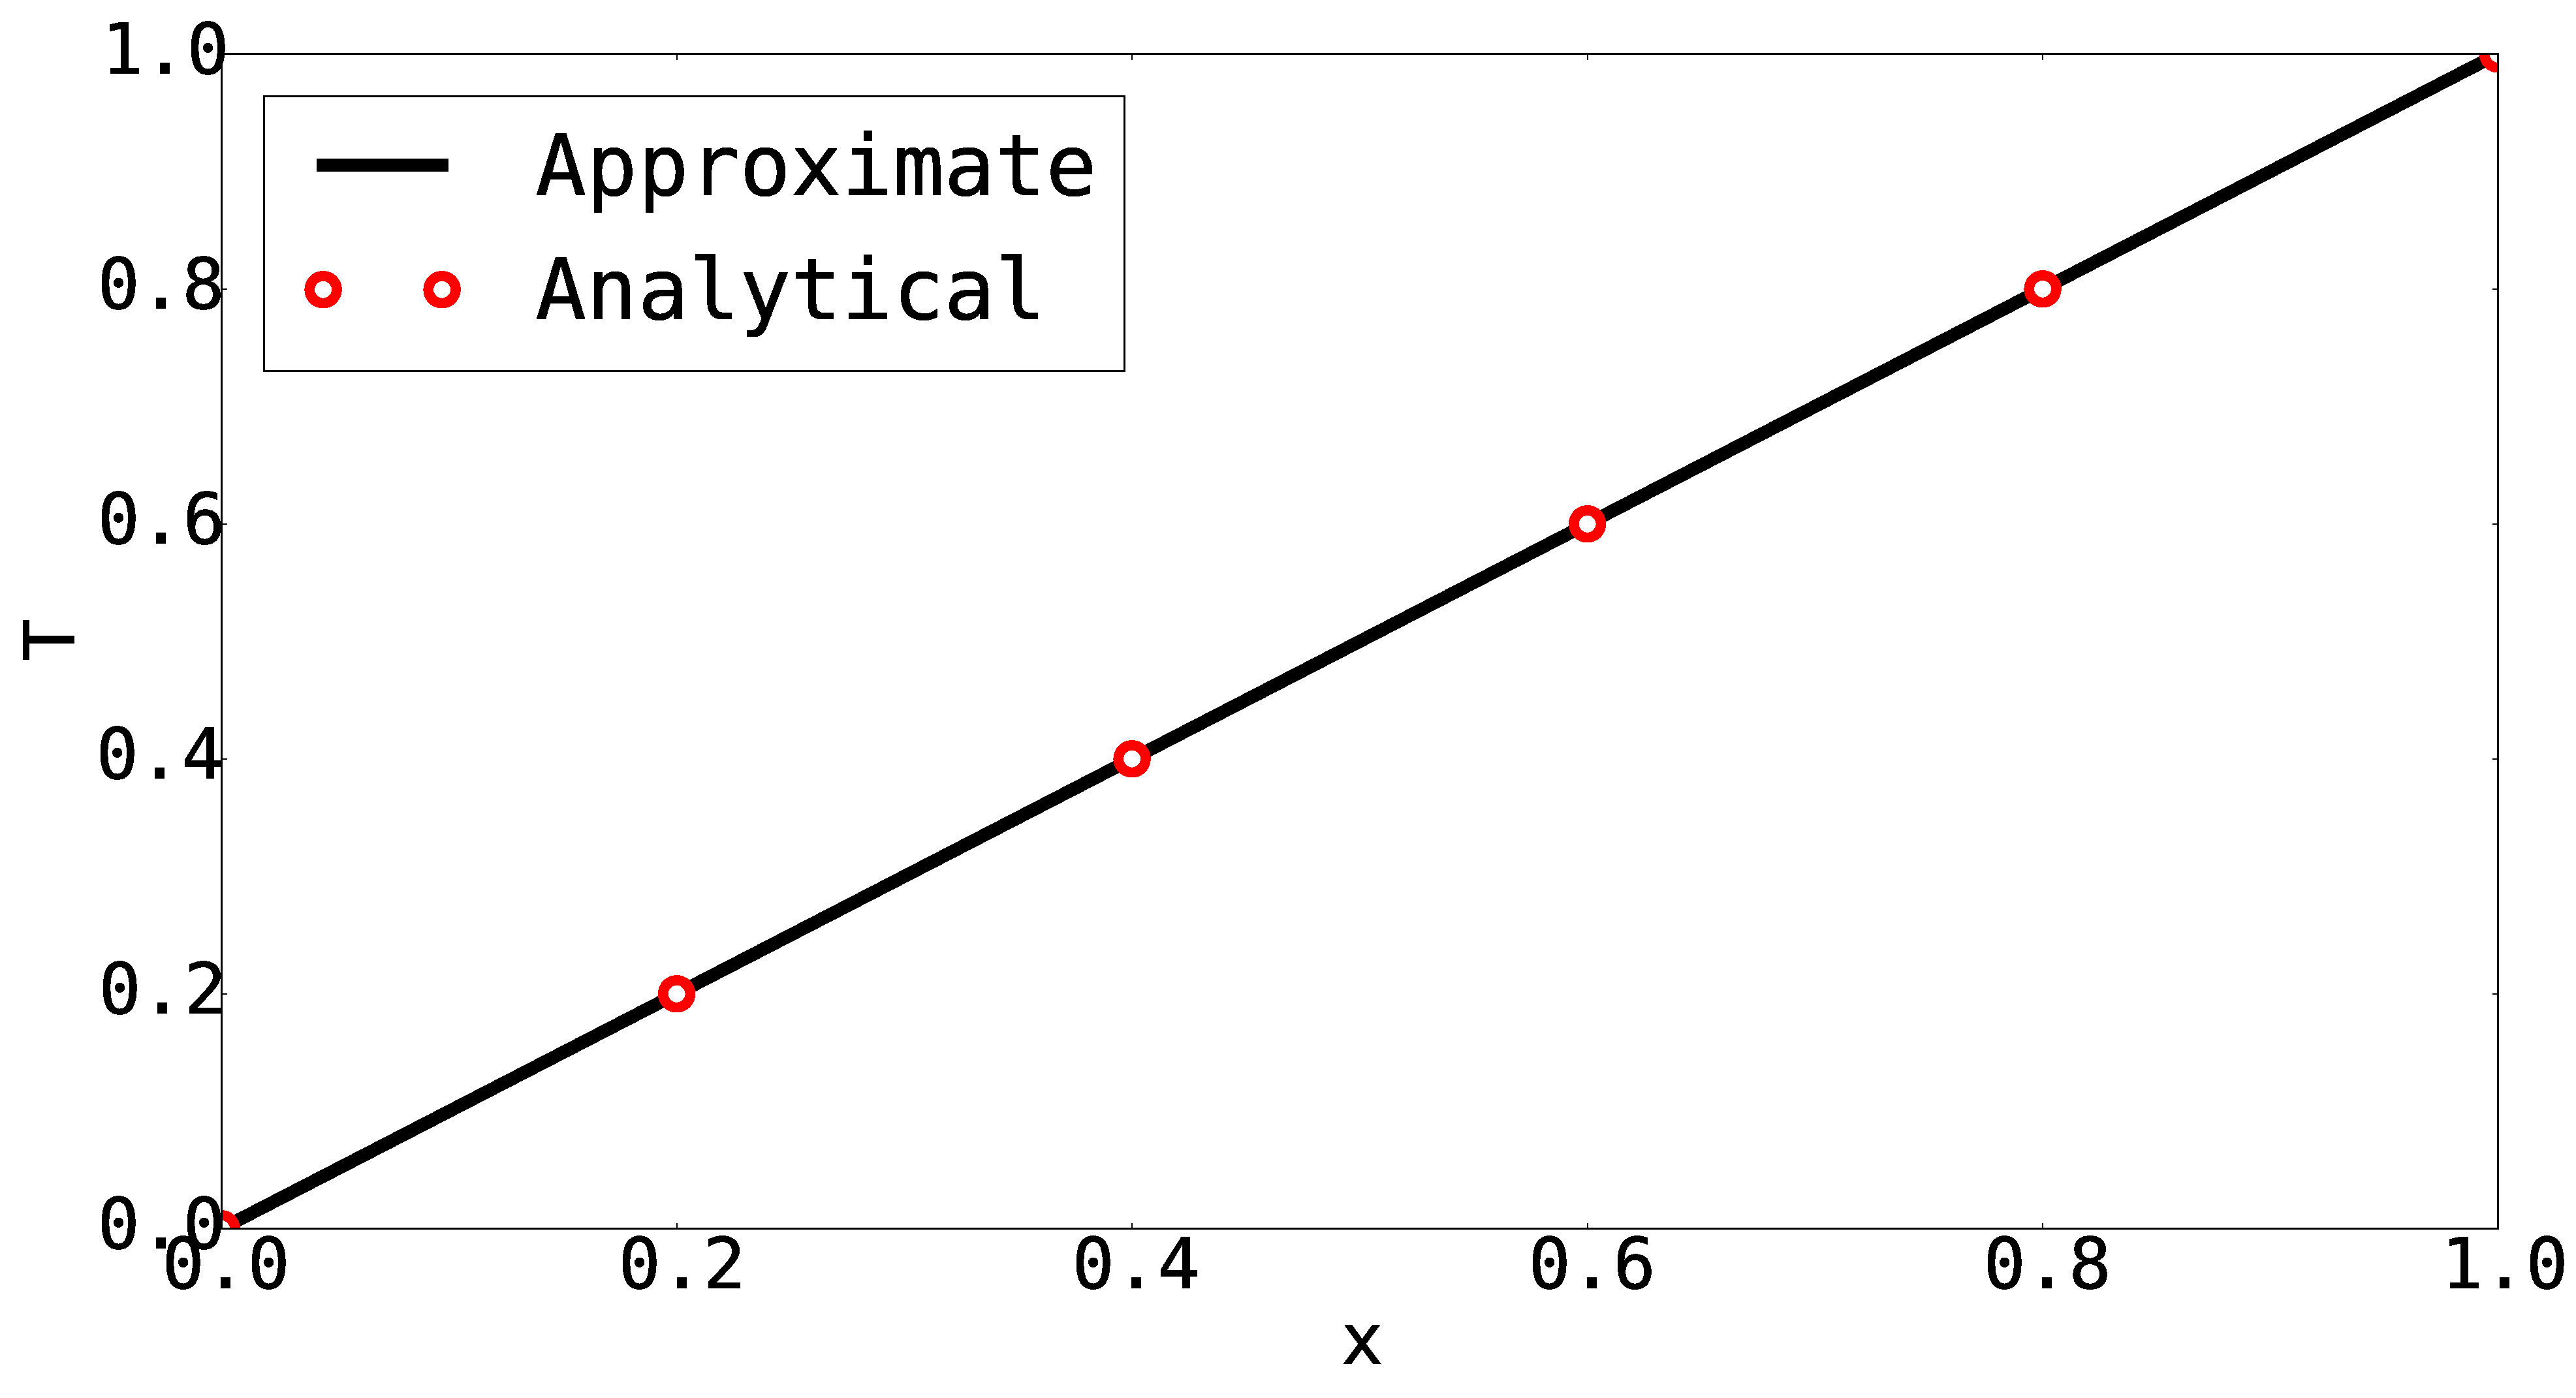
\includegraphics[width=6.5cm]{Chapter_2/figure/finitedifference_vs_analytical_n6.eps}
    }
    \quad
    \subfigure[$n = 12$]
    {
    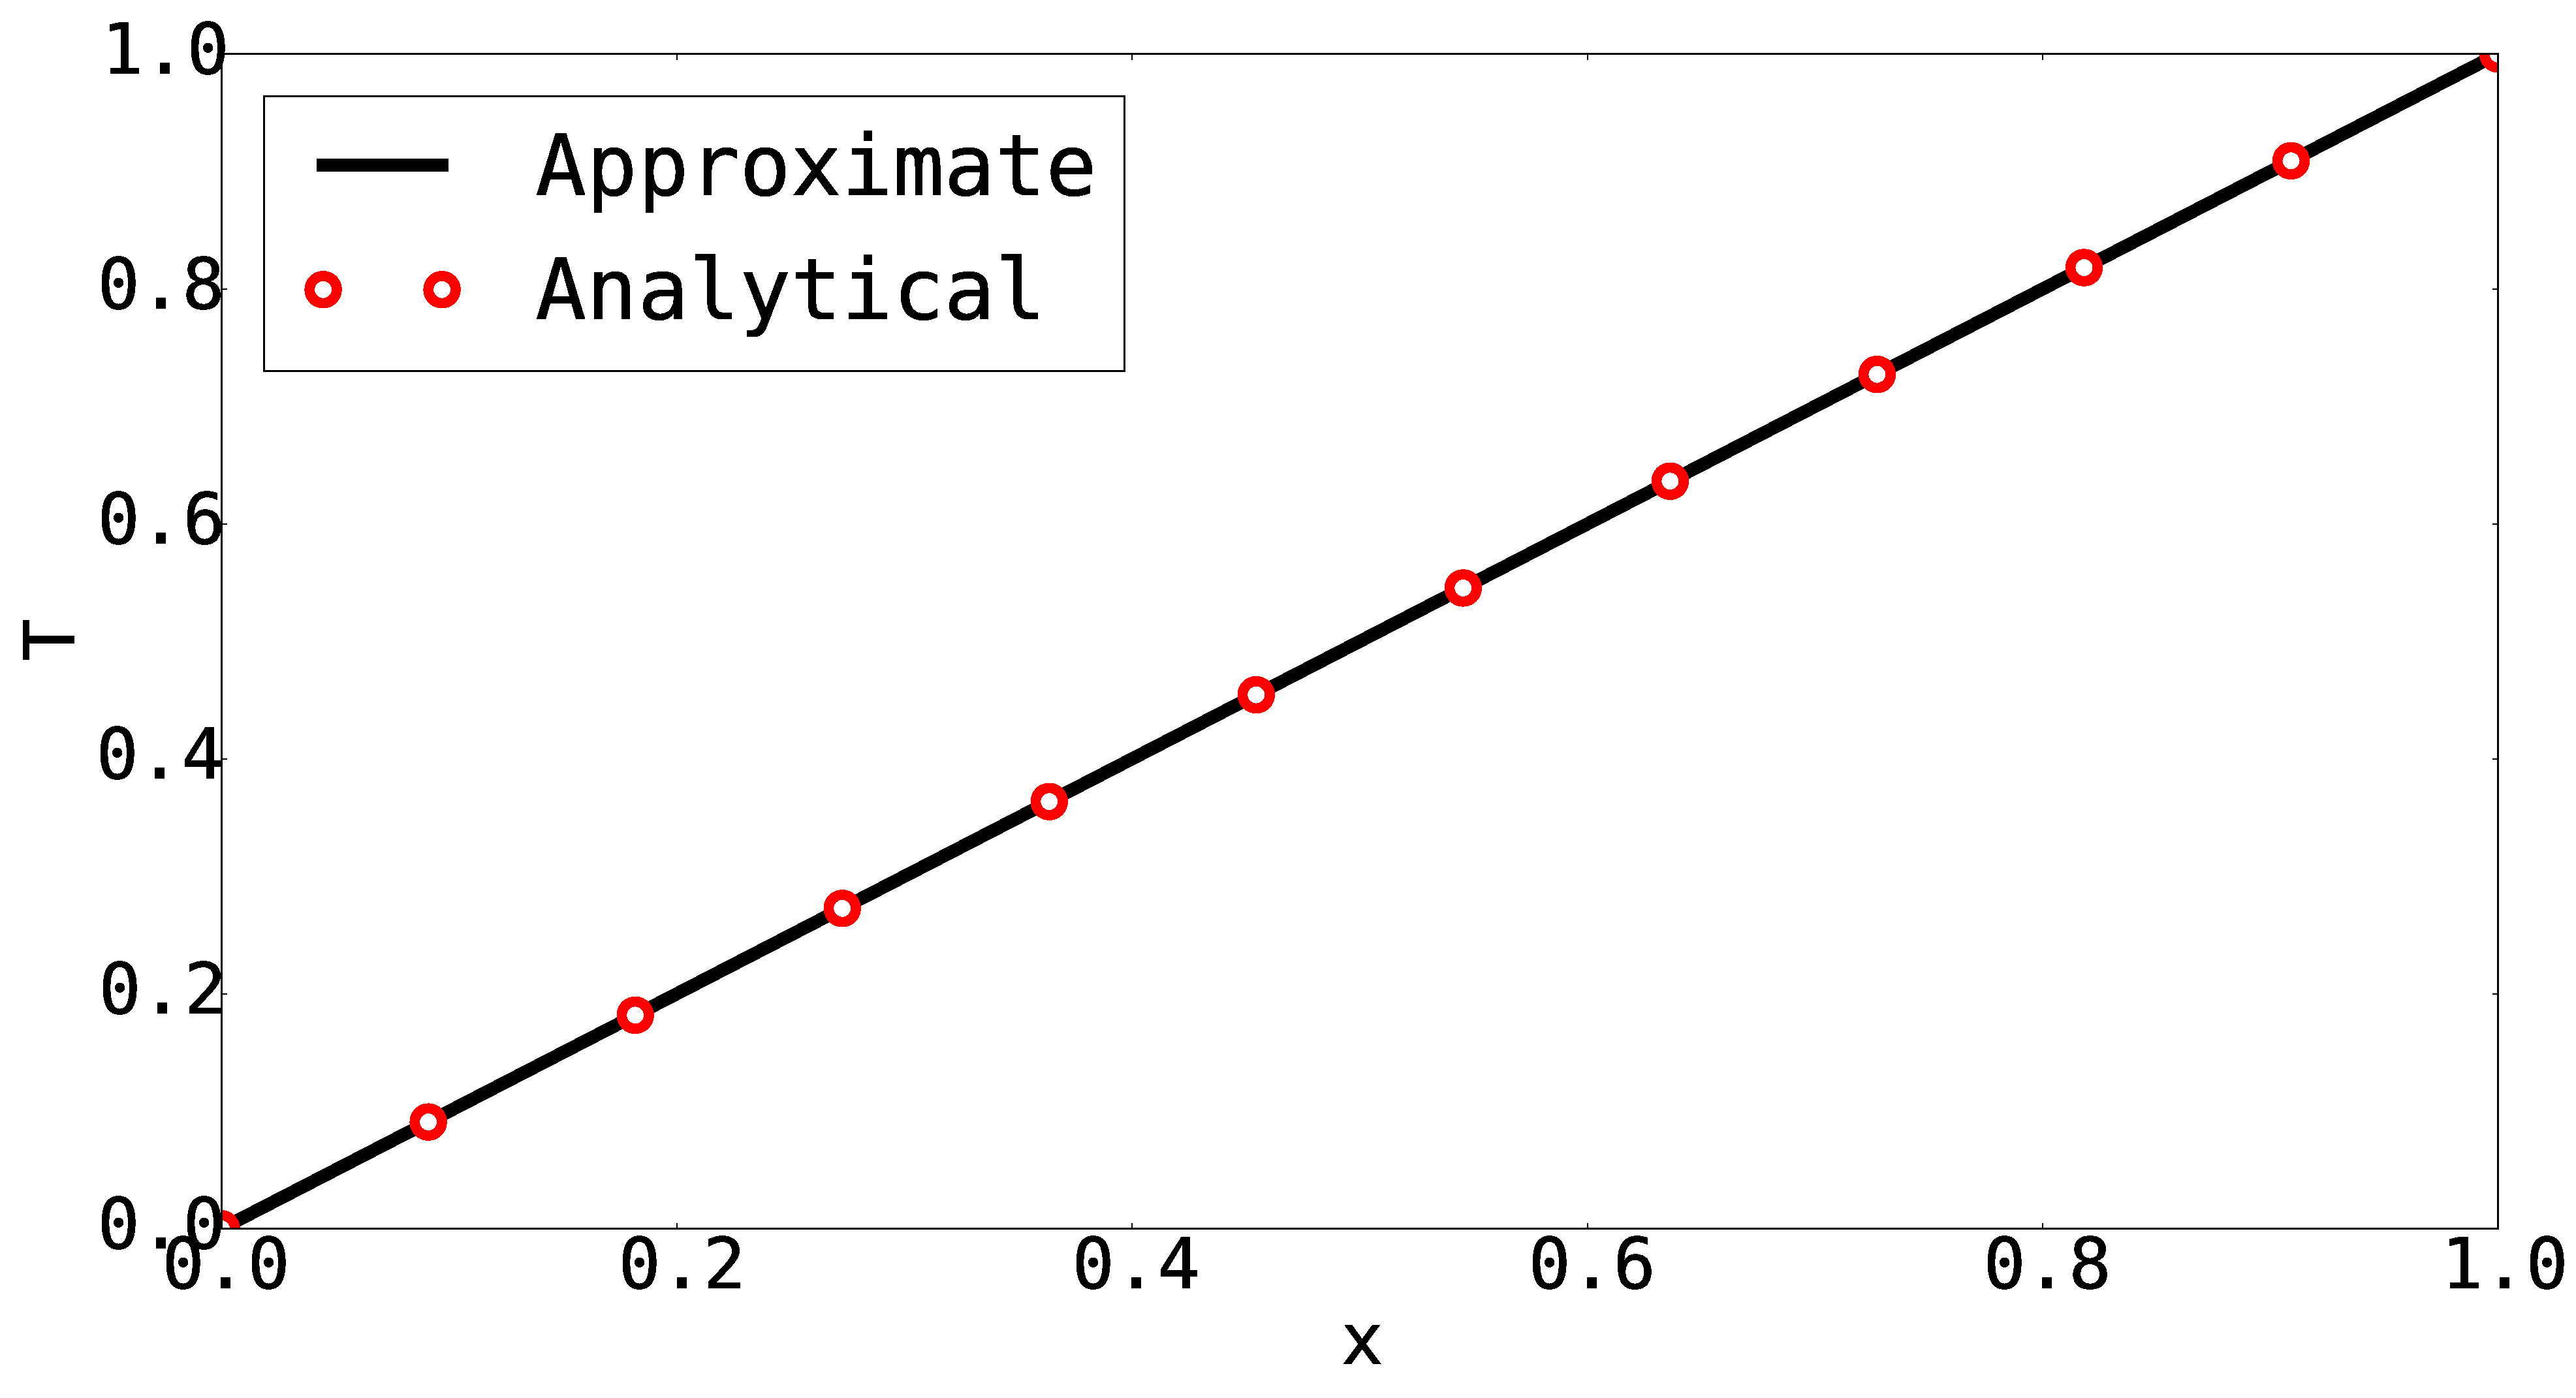
\includegraphics[width=6.5cm]{Chapter_2/figure/finitedifference_vs_analytical_n12.eps}
    }
    \\
    \subfigure[$n = 24$]
    {
    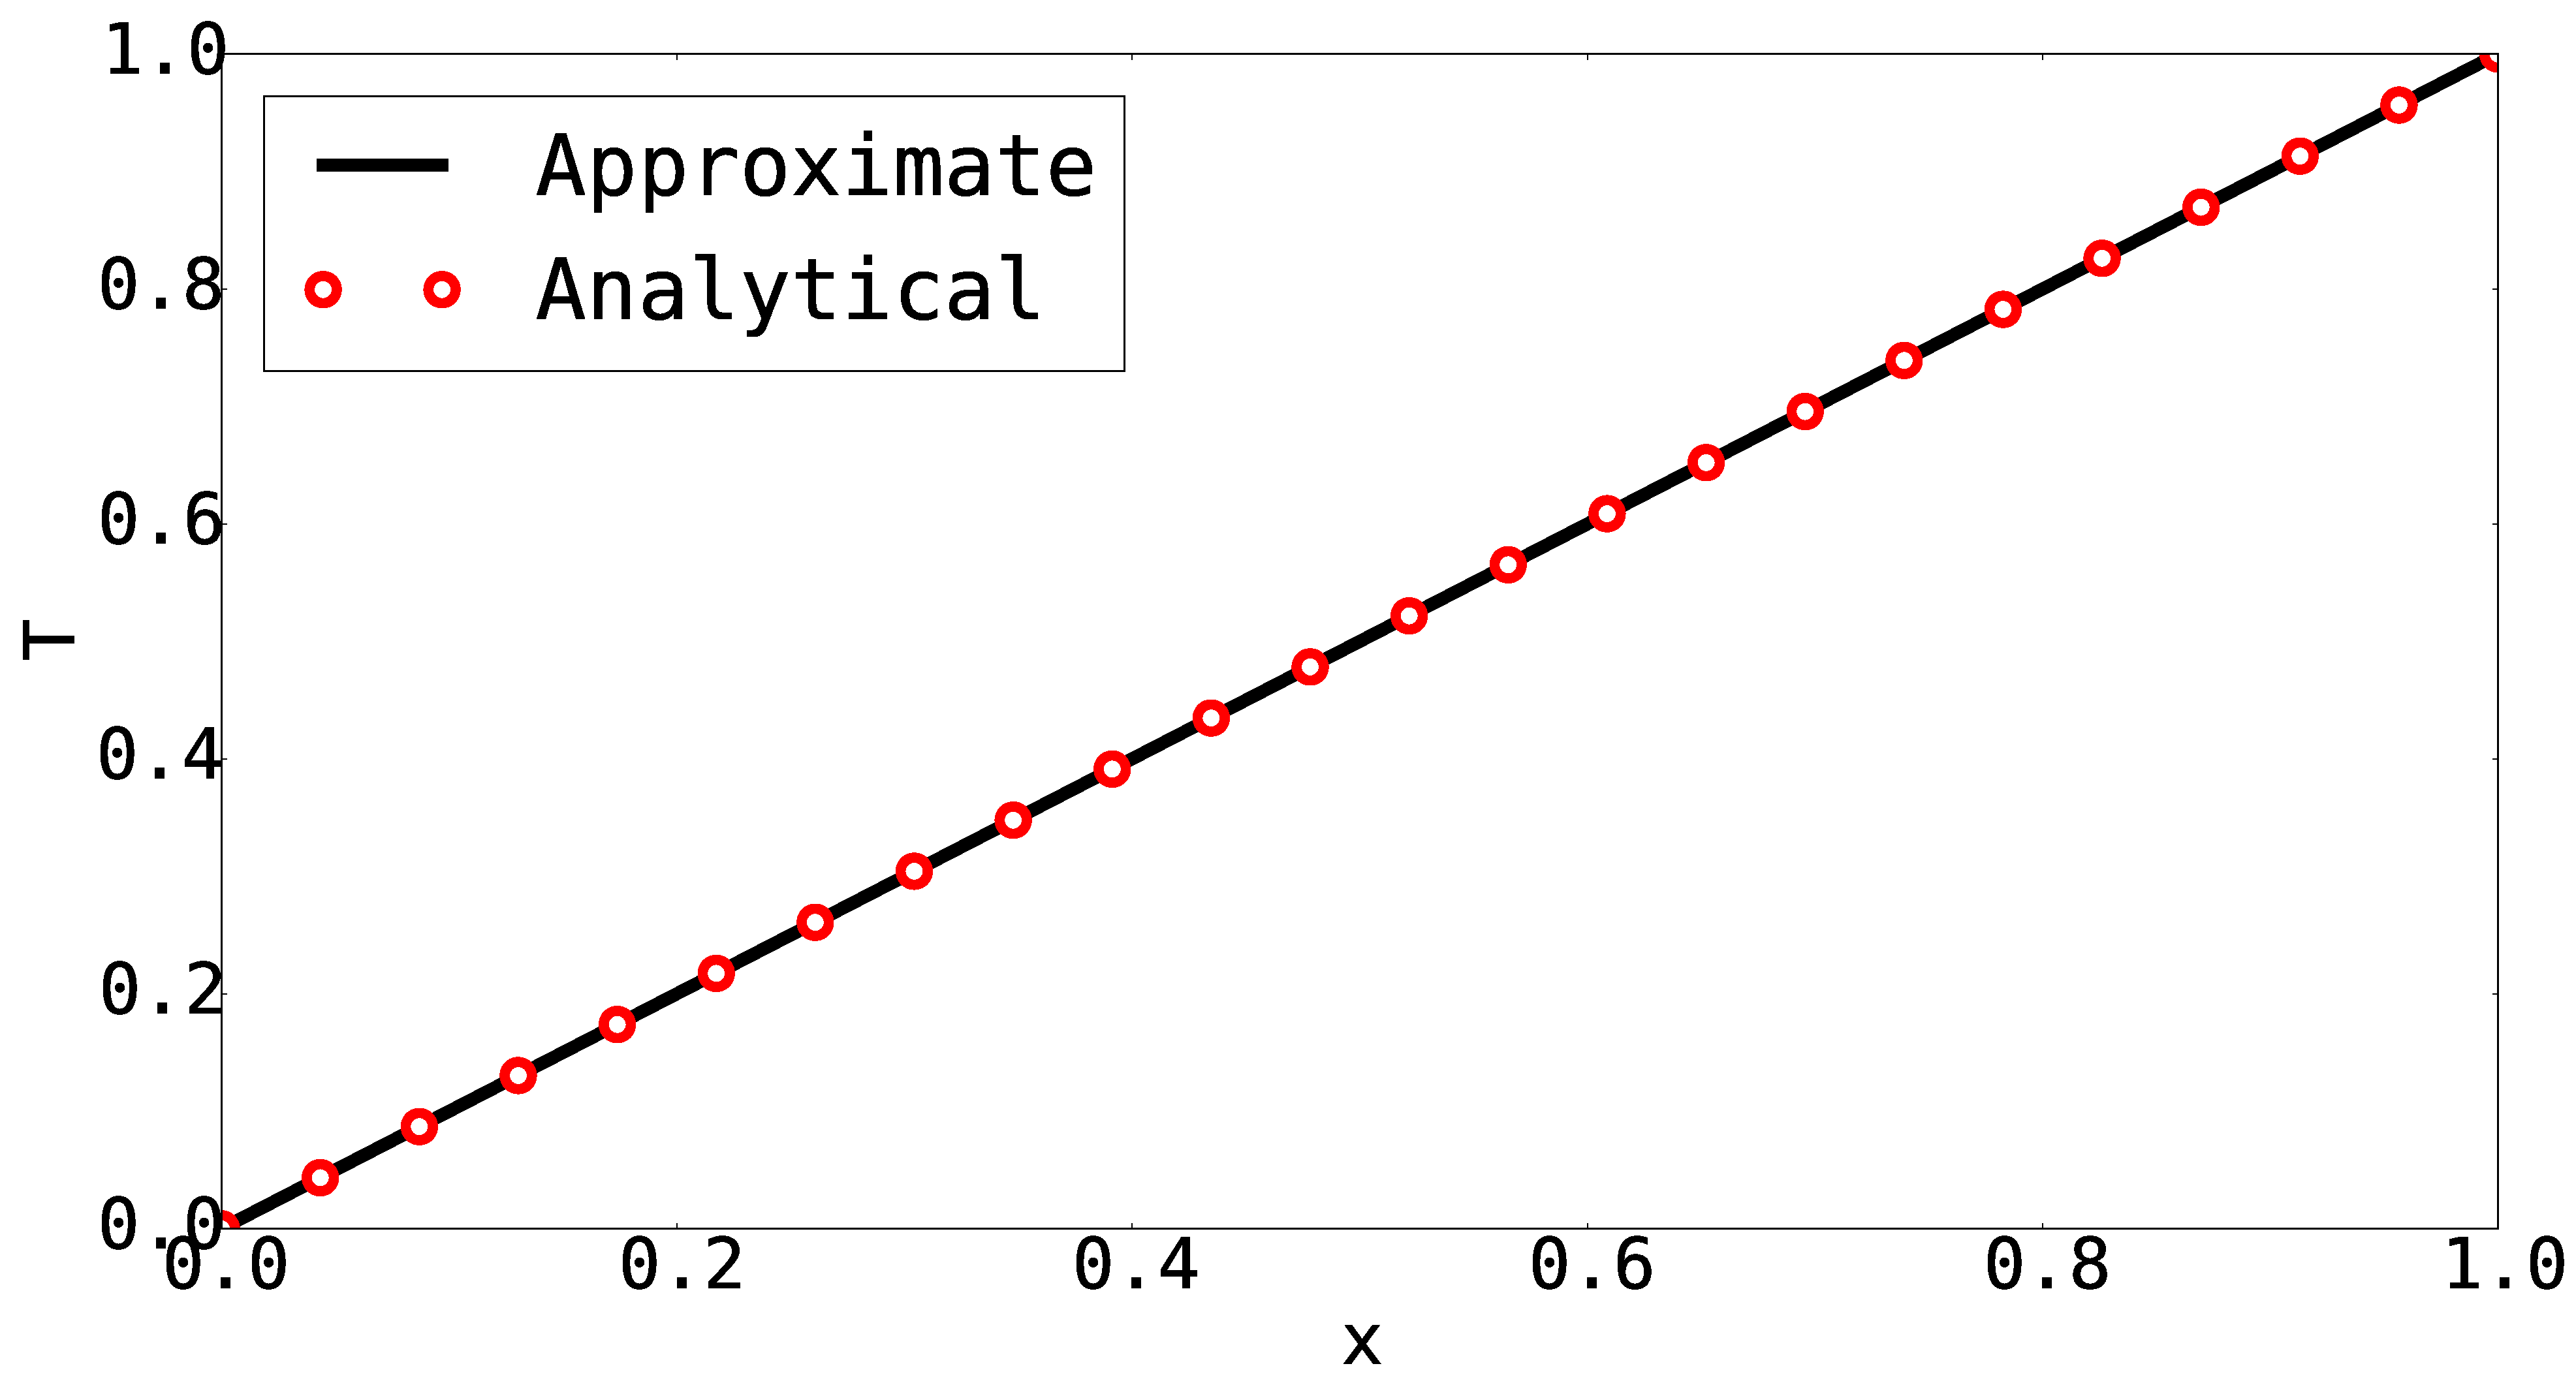
\includegraphics[width=6.5cm]{Chapter_2/figure/finitedifference_vs_analytical_n24.eps}
    }
    \quad
    \subfigure[$n = 48$]
    {
    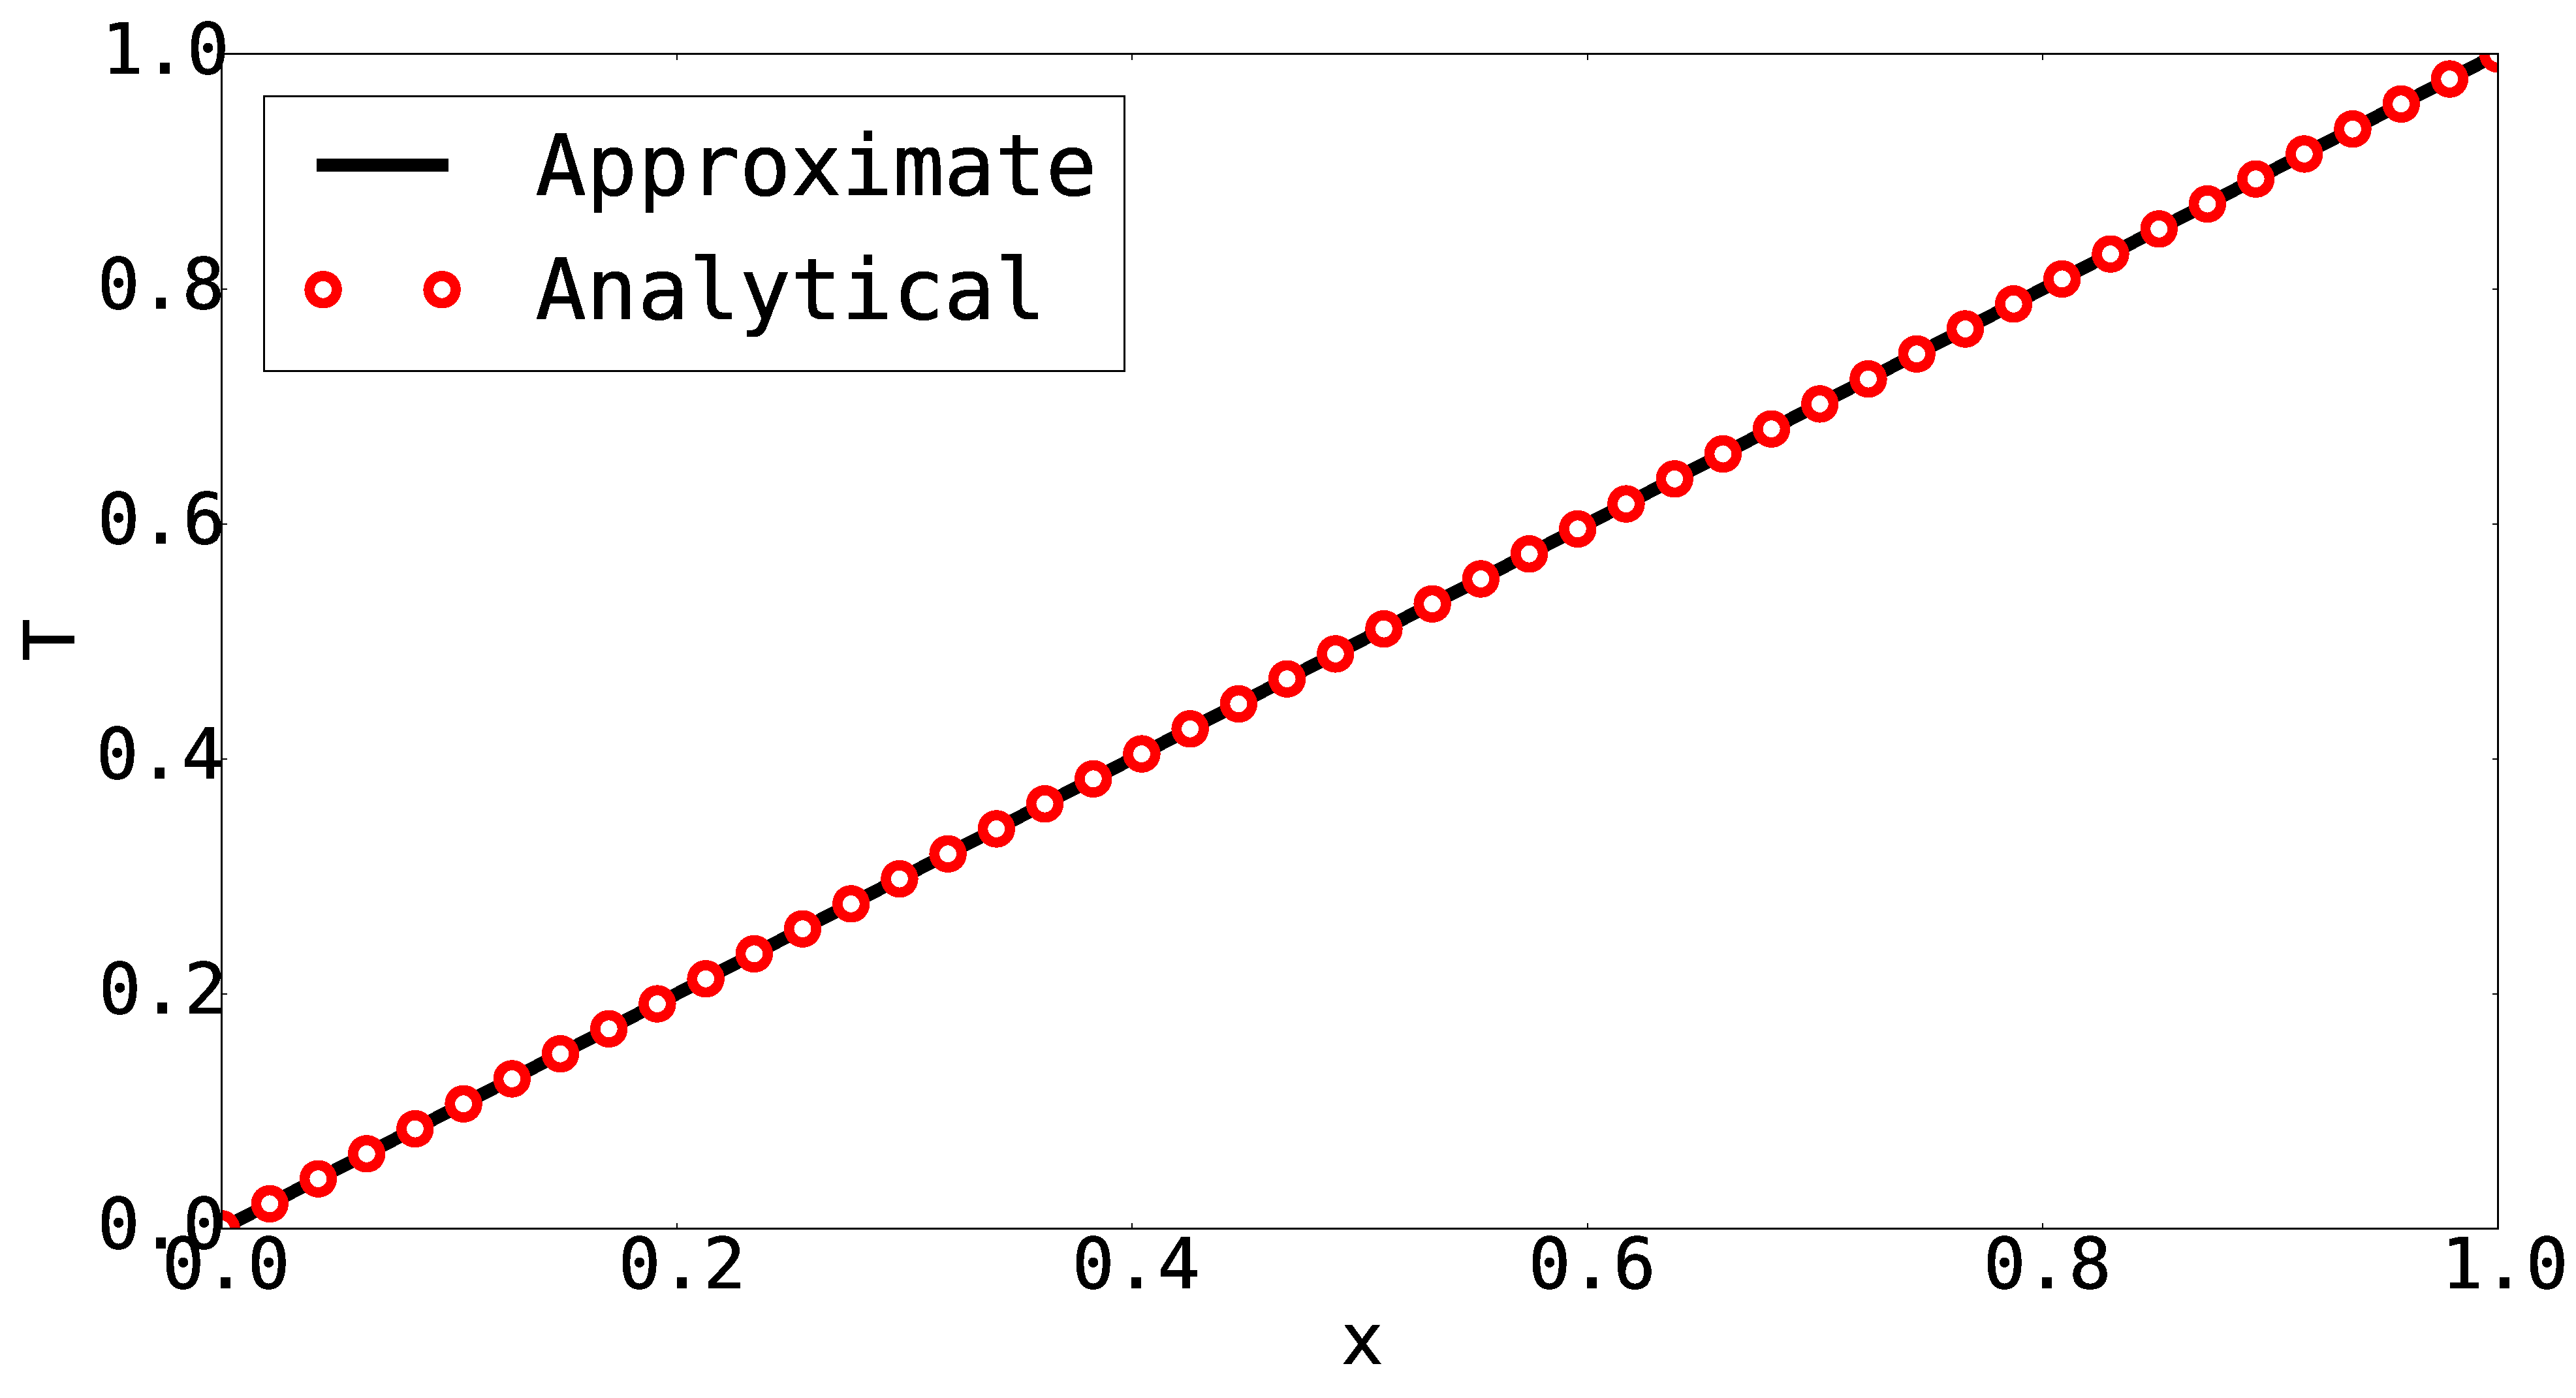
\includegraphics[width=6.5cm]{Chapter_2/figure/finitedifference_vs_analytical_n48.eps}
    }
    \caption{Comparison between the analytical and finite difference solutions for 1D heat equation for different number of nodes.}
    \label{fig:C2_verificationOfSolver}
\end{figure}
%
%
\begin{table}[H]
\centering
\begin{tabular}{| c | c |}
    \hline
    Number of nodes & absolute error \\ \hline \hline
    6 & $1.85 \times 10^{-16}$ \\ \hline
    12 & $2.03 \times 10^{-16}$ \\ \hline
    24 & $1.27 \times 10^{-15}$ \\ \hline
    48 & $8.55 \times 10^{-15}$ \\ \hline
\end{tabular}
\caption{Absolute error value for different number of nodes.}
\label{table:C2_solutionError}
\end{table}
%
The discrete sensitivity equations are derived by differentiating the discretized governing equation of \eqref{eq:C2_laplaceEquationMatrixForm} to the length of the domain. We assume that the change in the length only affects the nodal distance between the last two nodes and the rest remain unchanged. This means that only the node next to the boundary will move, and the rest of nodes will be stationary. This is required to make sure that the sensitivity at each of the degrees of freedom is only a function of the change in shape not the movement of material nodes; therefore, $\partial x/\partial b$ is equal to zero.

In order to differentiate Equation  \eqref{eq:C2_laplaceEquationMatrixForm}, it is required to calculate the derivative of nodal distances in Equation \eqref{eq:C2_laplaceEquationMatrixForm} with respect to $L$, $\partial \Delta_i/\partial L$. For an equally spaced grid, the nodal distance is written as
%
\begin{equation*}
    \Delta = \frac{L}{n - 1}
\end{equation*}
%
Where $L$ is the length of the domain and $n$ is the number of nodes used to discretize the domain. Therefore, the sensitivity of nodal distances to the length of the domain is calculated as:
%
\begin{equation}\label{eq:C2_nodeDistanceSensitivity}
    \frac{\partial \Delta}{\partial L} = \frac{1}{n-1}
\end{equation}
%
The differentiated form of the discretized Equation \eqref{eq:C2_laplaceEquationMatrixForm} is written as
%
\begin{equation}\label{eq:C2_laplaceEquationMatrixFormSensitivity}
    \begin{bmatrix}
        -2 & 1 & 0 & 0 \\
        1 & -2 & 1 & 0 \\
        0 & 1 & -2 & 1 \\
        0 & 0 & 1 & -2
    \end{bmatrix}
    \begin{bmatrix}
        T'_2 \\
        T'_3 \\
        T'_4 \\
        T'_5
    \end{bmatrix}
    =
    \frac{1}{2} \frac{\partial \Delta}{\partial L} \frac{1}{\Delta}
    \begin{bmatrix}
        0 \\
        0 \\
        0 \\
        T_6
    \end{bmatrix}
    -
    \underbrace{
    \frac{1}{2} \frac{\partial \Delta}{\partial L} \frac{1}{\Delta}
    \begin{bmatrix}
        0 & 0 & 0 & 0 \\
        0 & 0 & 0 & 0 \\
        0 & 0 & 0 & 0 \\
        0 & 0 & -3 & 1
    \end{bmatrix}
    \begin{bmatrix}
        T_2 \\
        T_3 \\
        T_4 \\
        T_5
    \end{bmatrix}}_\text{effect of shape change}
\end{equation}
%
It should be noted that since only the adjacent node to the boundary is affected by shape change, only that element in the matrix derivative has a value. $T^\prime_i$ represents the sensitivity of temperature to length of the domain.

To verify the results of Equation \eqref{eq:C2_laplaceEquationMatrixFormSensitivity}, we compared it with the analytical sensitivity results as shown in Figure \ref{fig:C2_discreteSensitivityVerification}. We discretized the domain using $11$, $41$, $81$, and $161$ nodes for this purpose; however, this does not affect the solution accuracy. We chose the normalized root-mean-square deviation (NRMSD) for comparing the sensitivity results. This is defined in Equation \eqref{eq:C2_NRMSD}.
%
\begin{equation}\label{eq:C2_NRMSD}
    NRMSD = \dfrac{\sqrt{\dfrac{\sum (\hat{y}_t - y)^2}{n}}}{y_{max} - y_{min}}
\end{equation}
%
Where $\hat{y}$ is the value calculated using DSA and $y$ is the true value calculated by the analytical equation. The results for the NRMSD for this problem using different numbers of nodes are shown in Table \ref{table:C2_DSA_NRMSD}.
%
\begin{figure}[H]
    \centering
    \subfigure[$n = 11$]
    {
    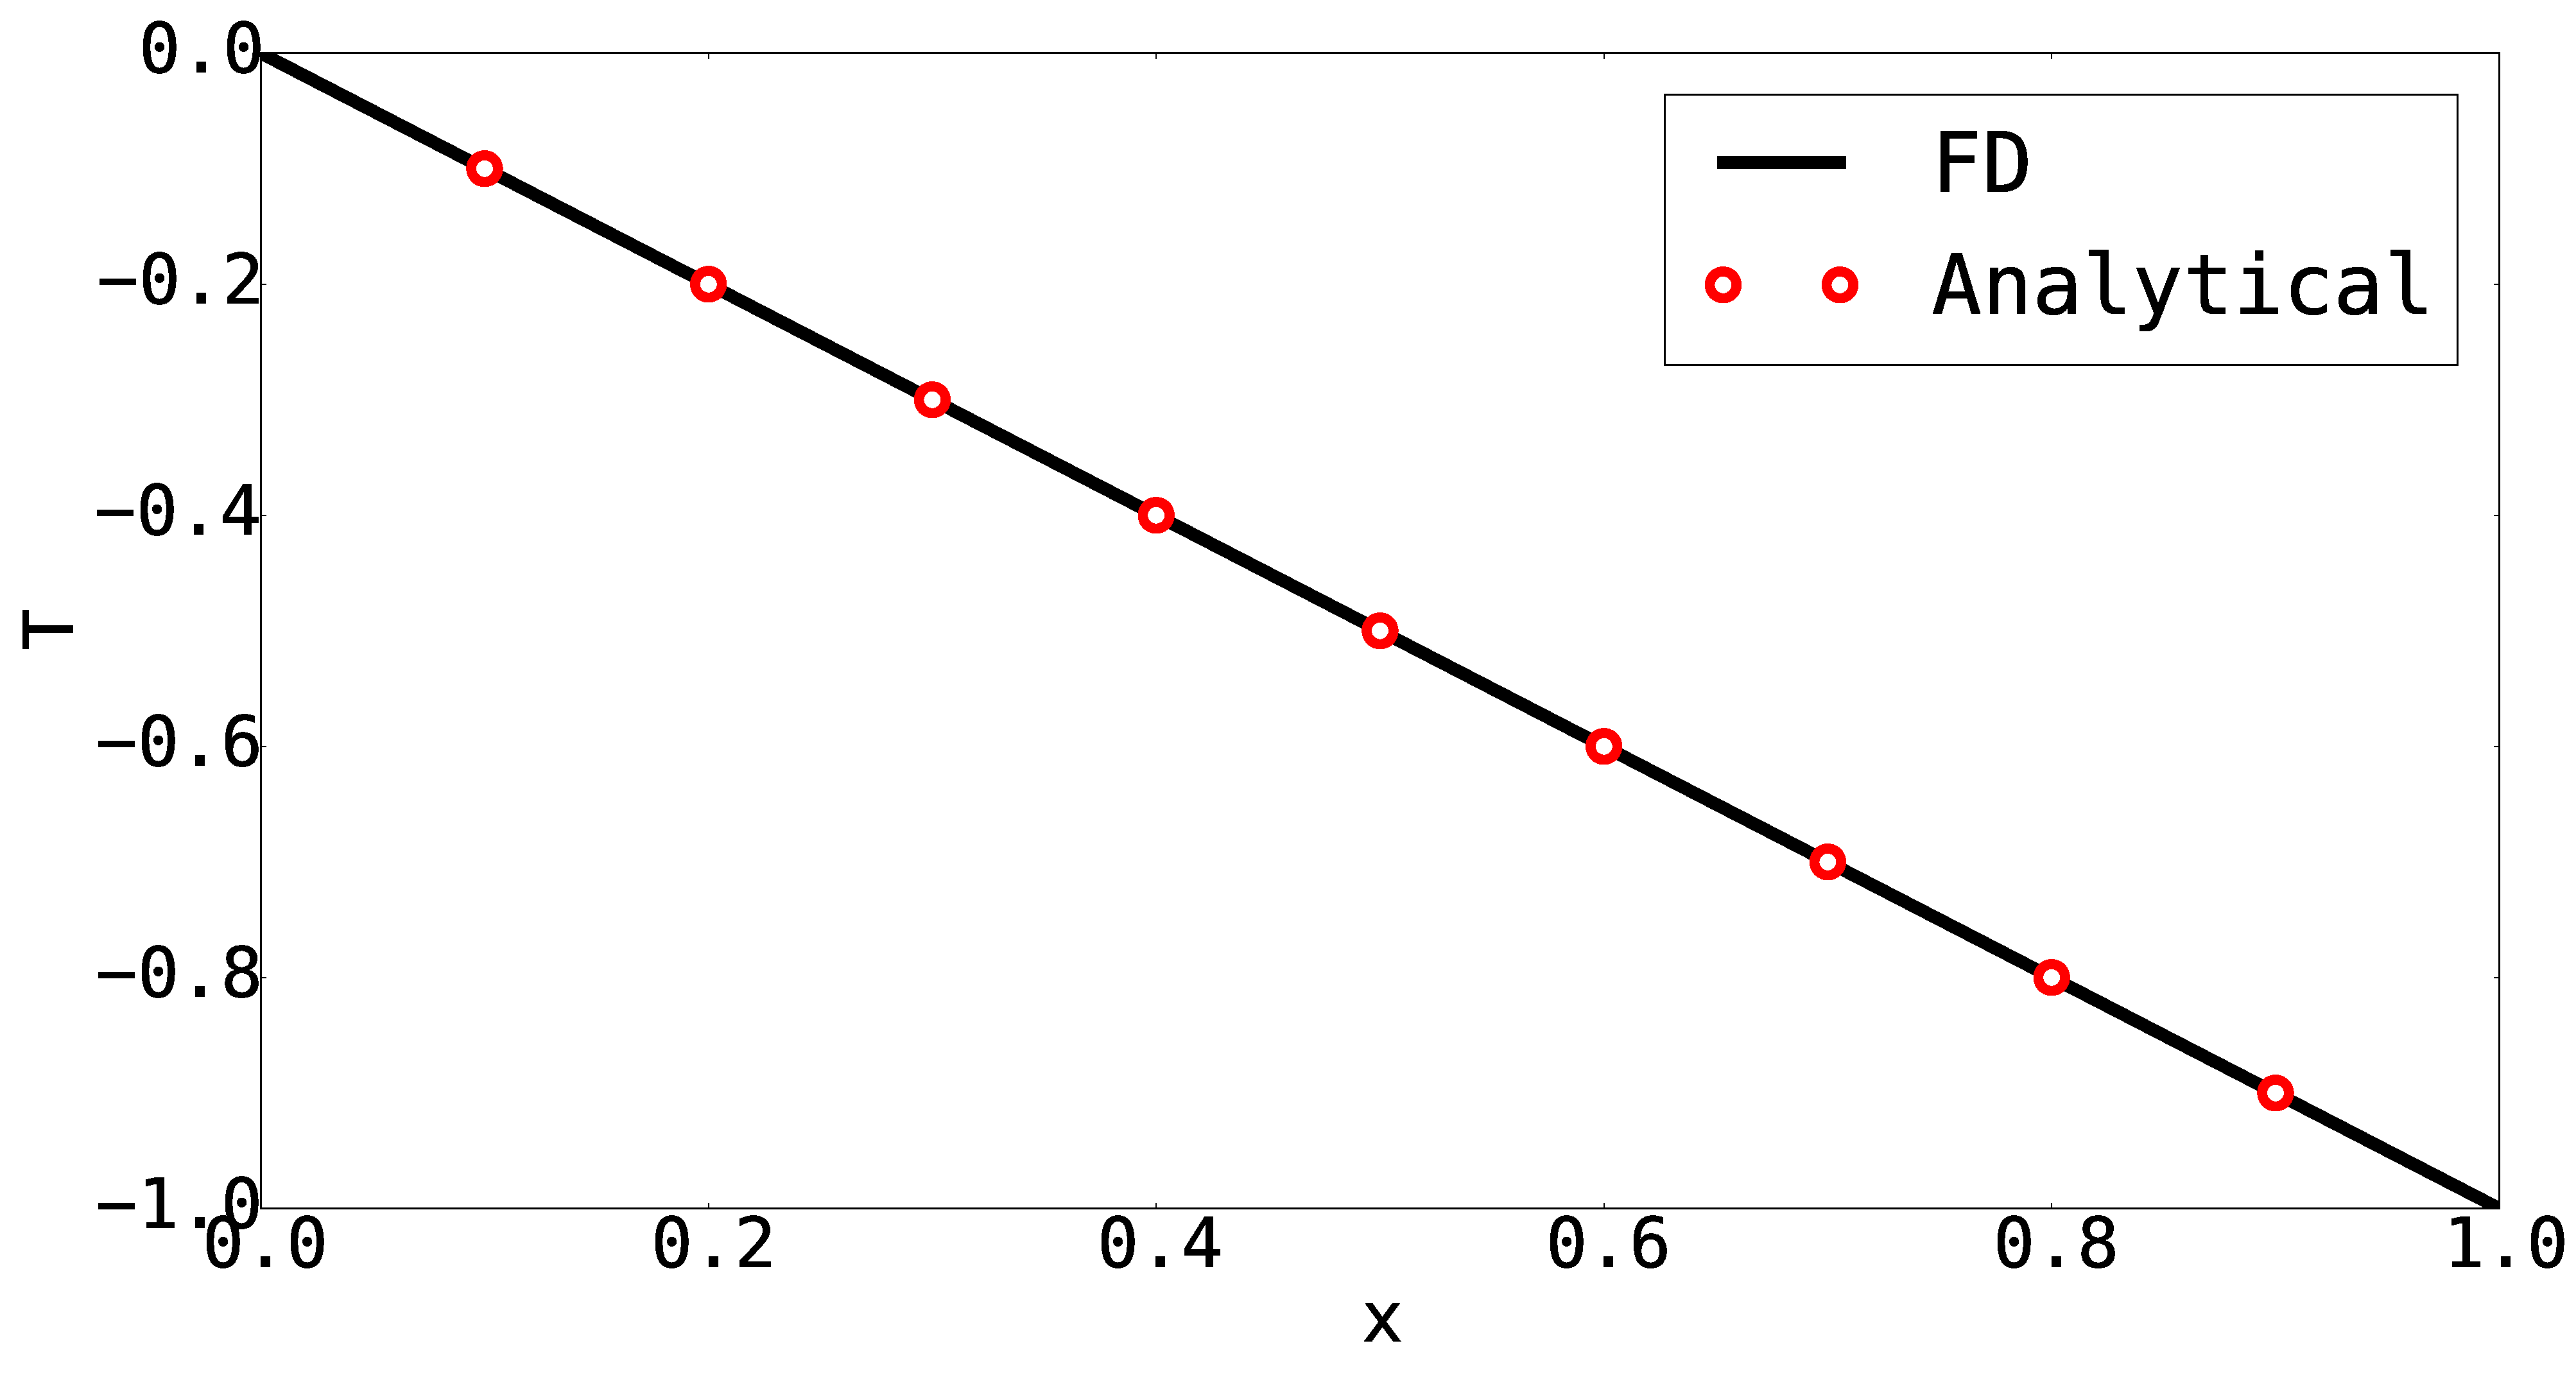
\includegraphics[width=6.5cm]{Chapter_2/figure/DSA_n11.eps}
    }
    \quad
    \subfigure[$n = 41$]
    {
    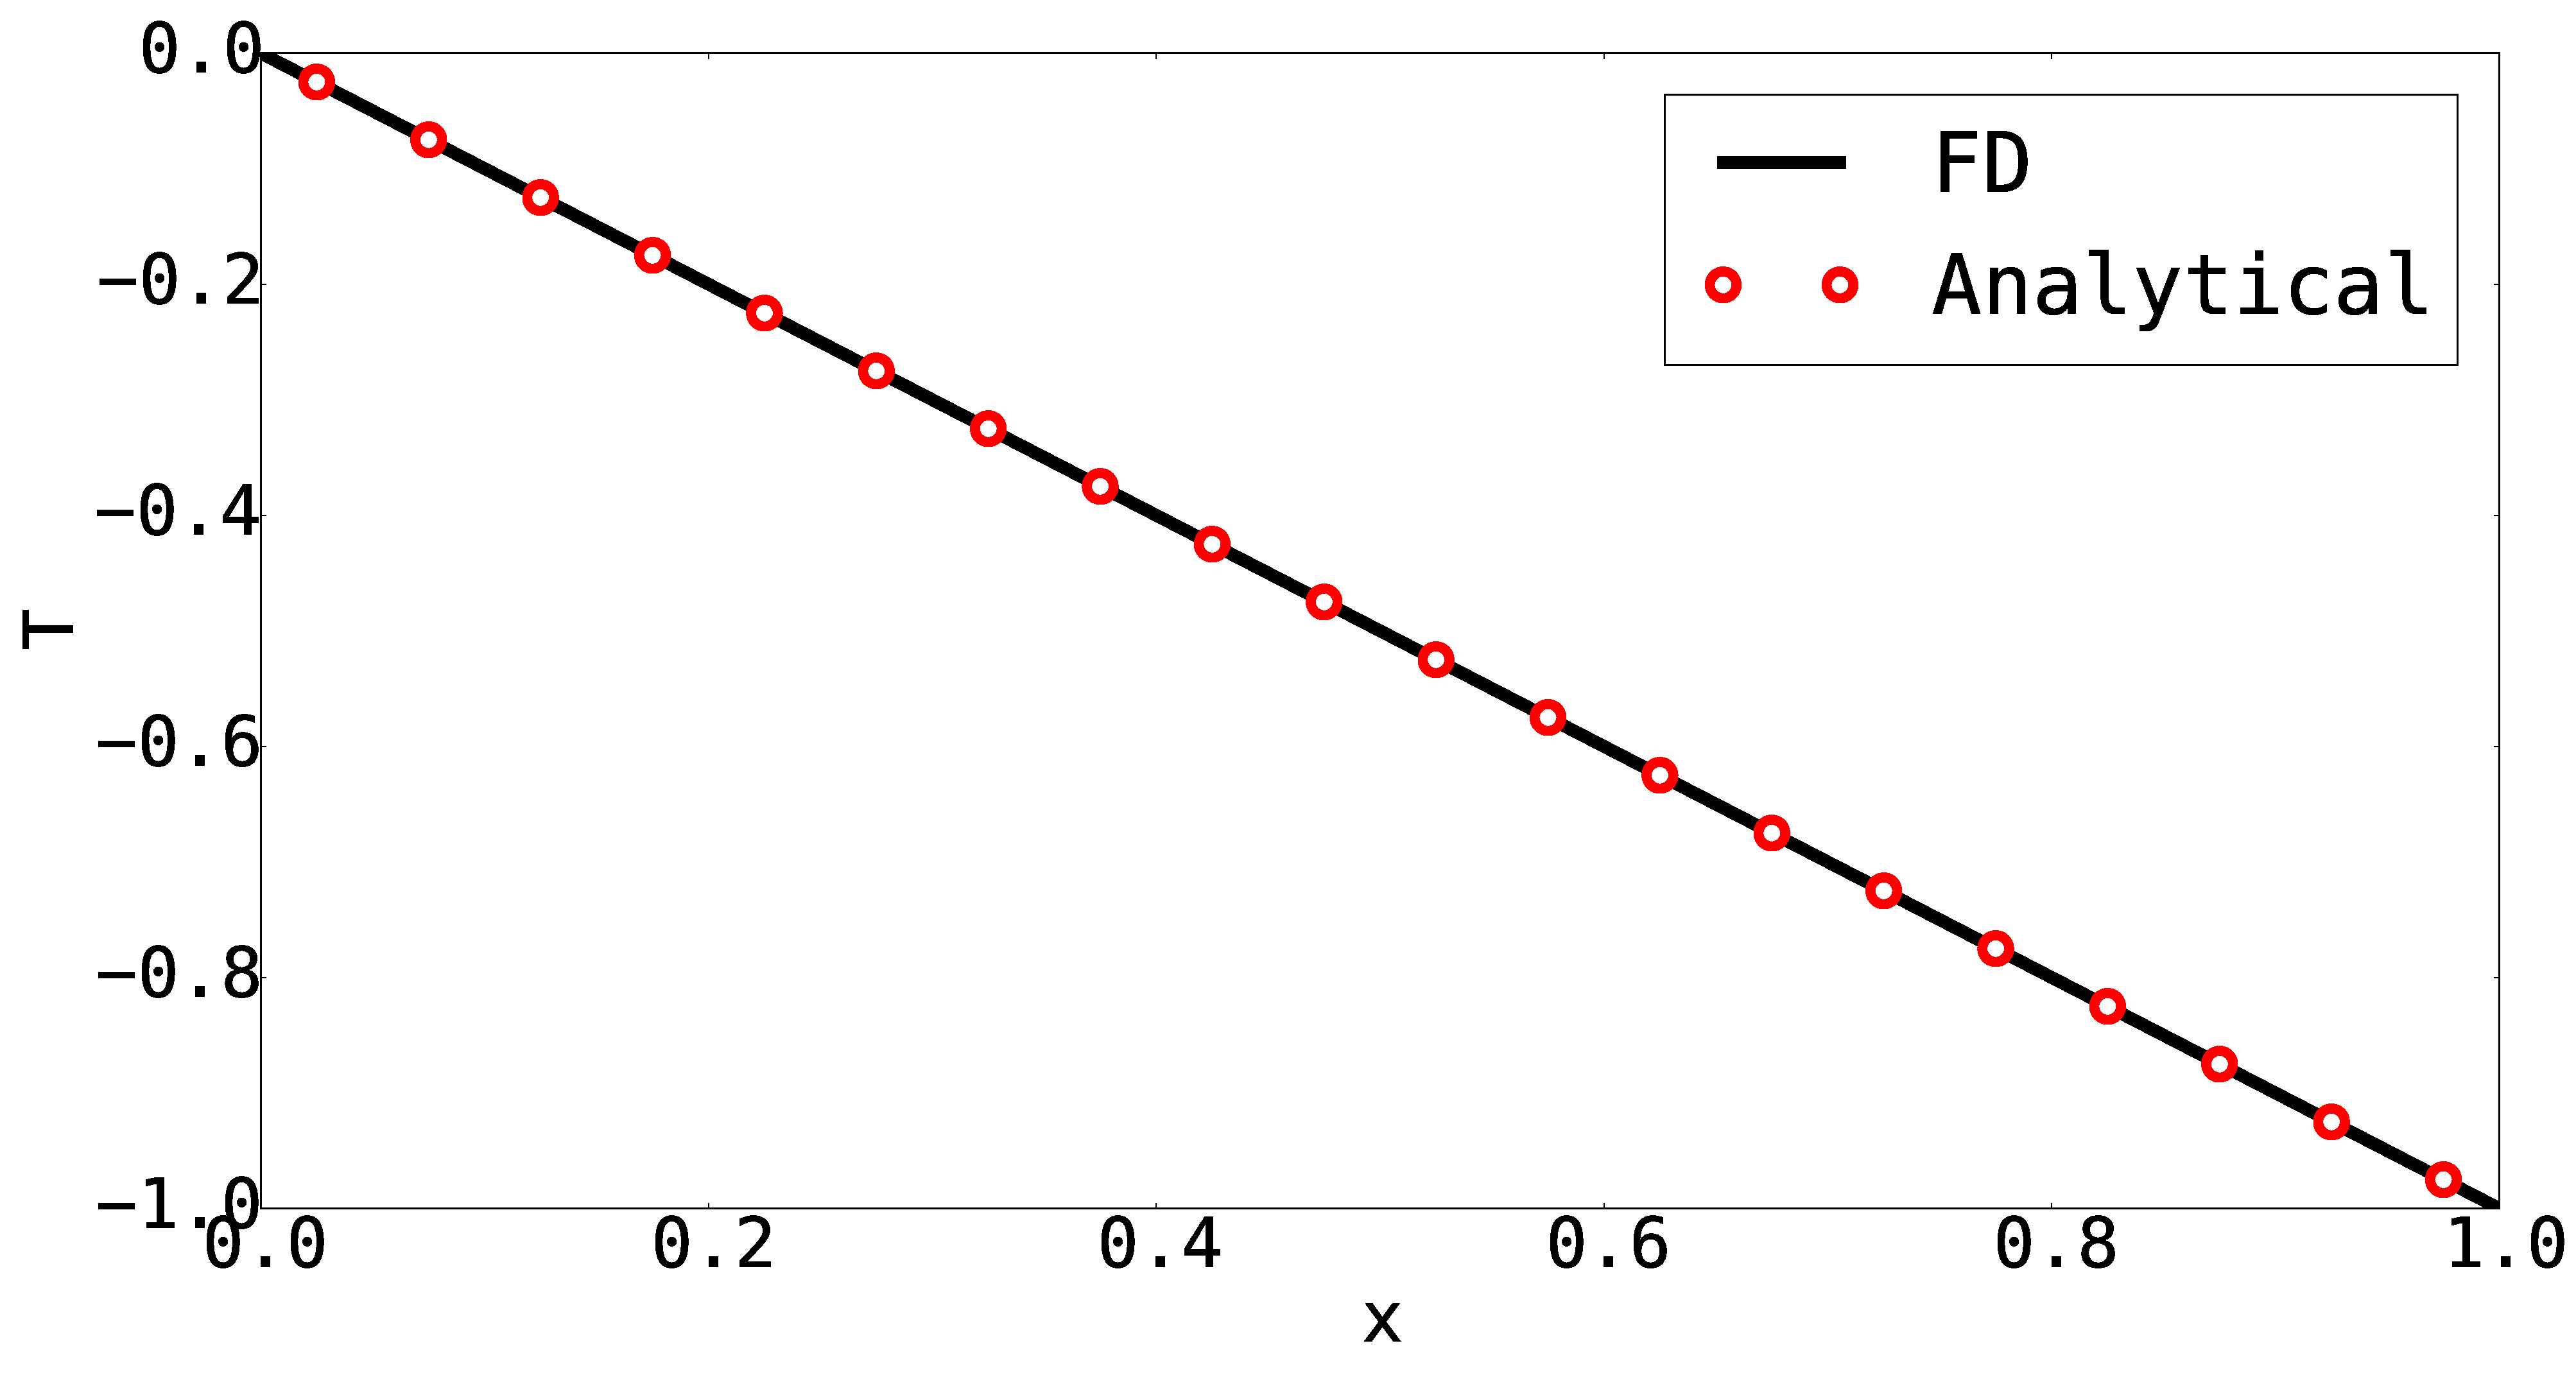
\includegraphics[width=6.5cm]{Chapter_2/figure/DSA_n41.eps}
    }
    \\
    \subfigure[$n = 81$]
    {
    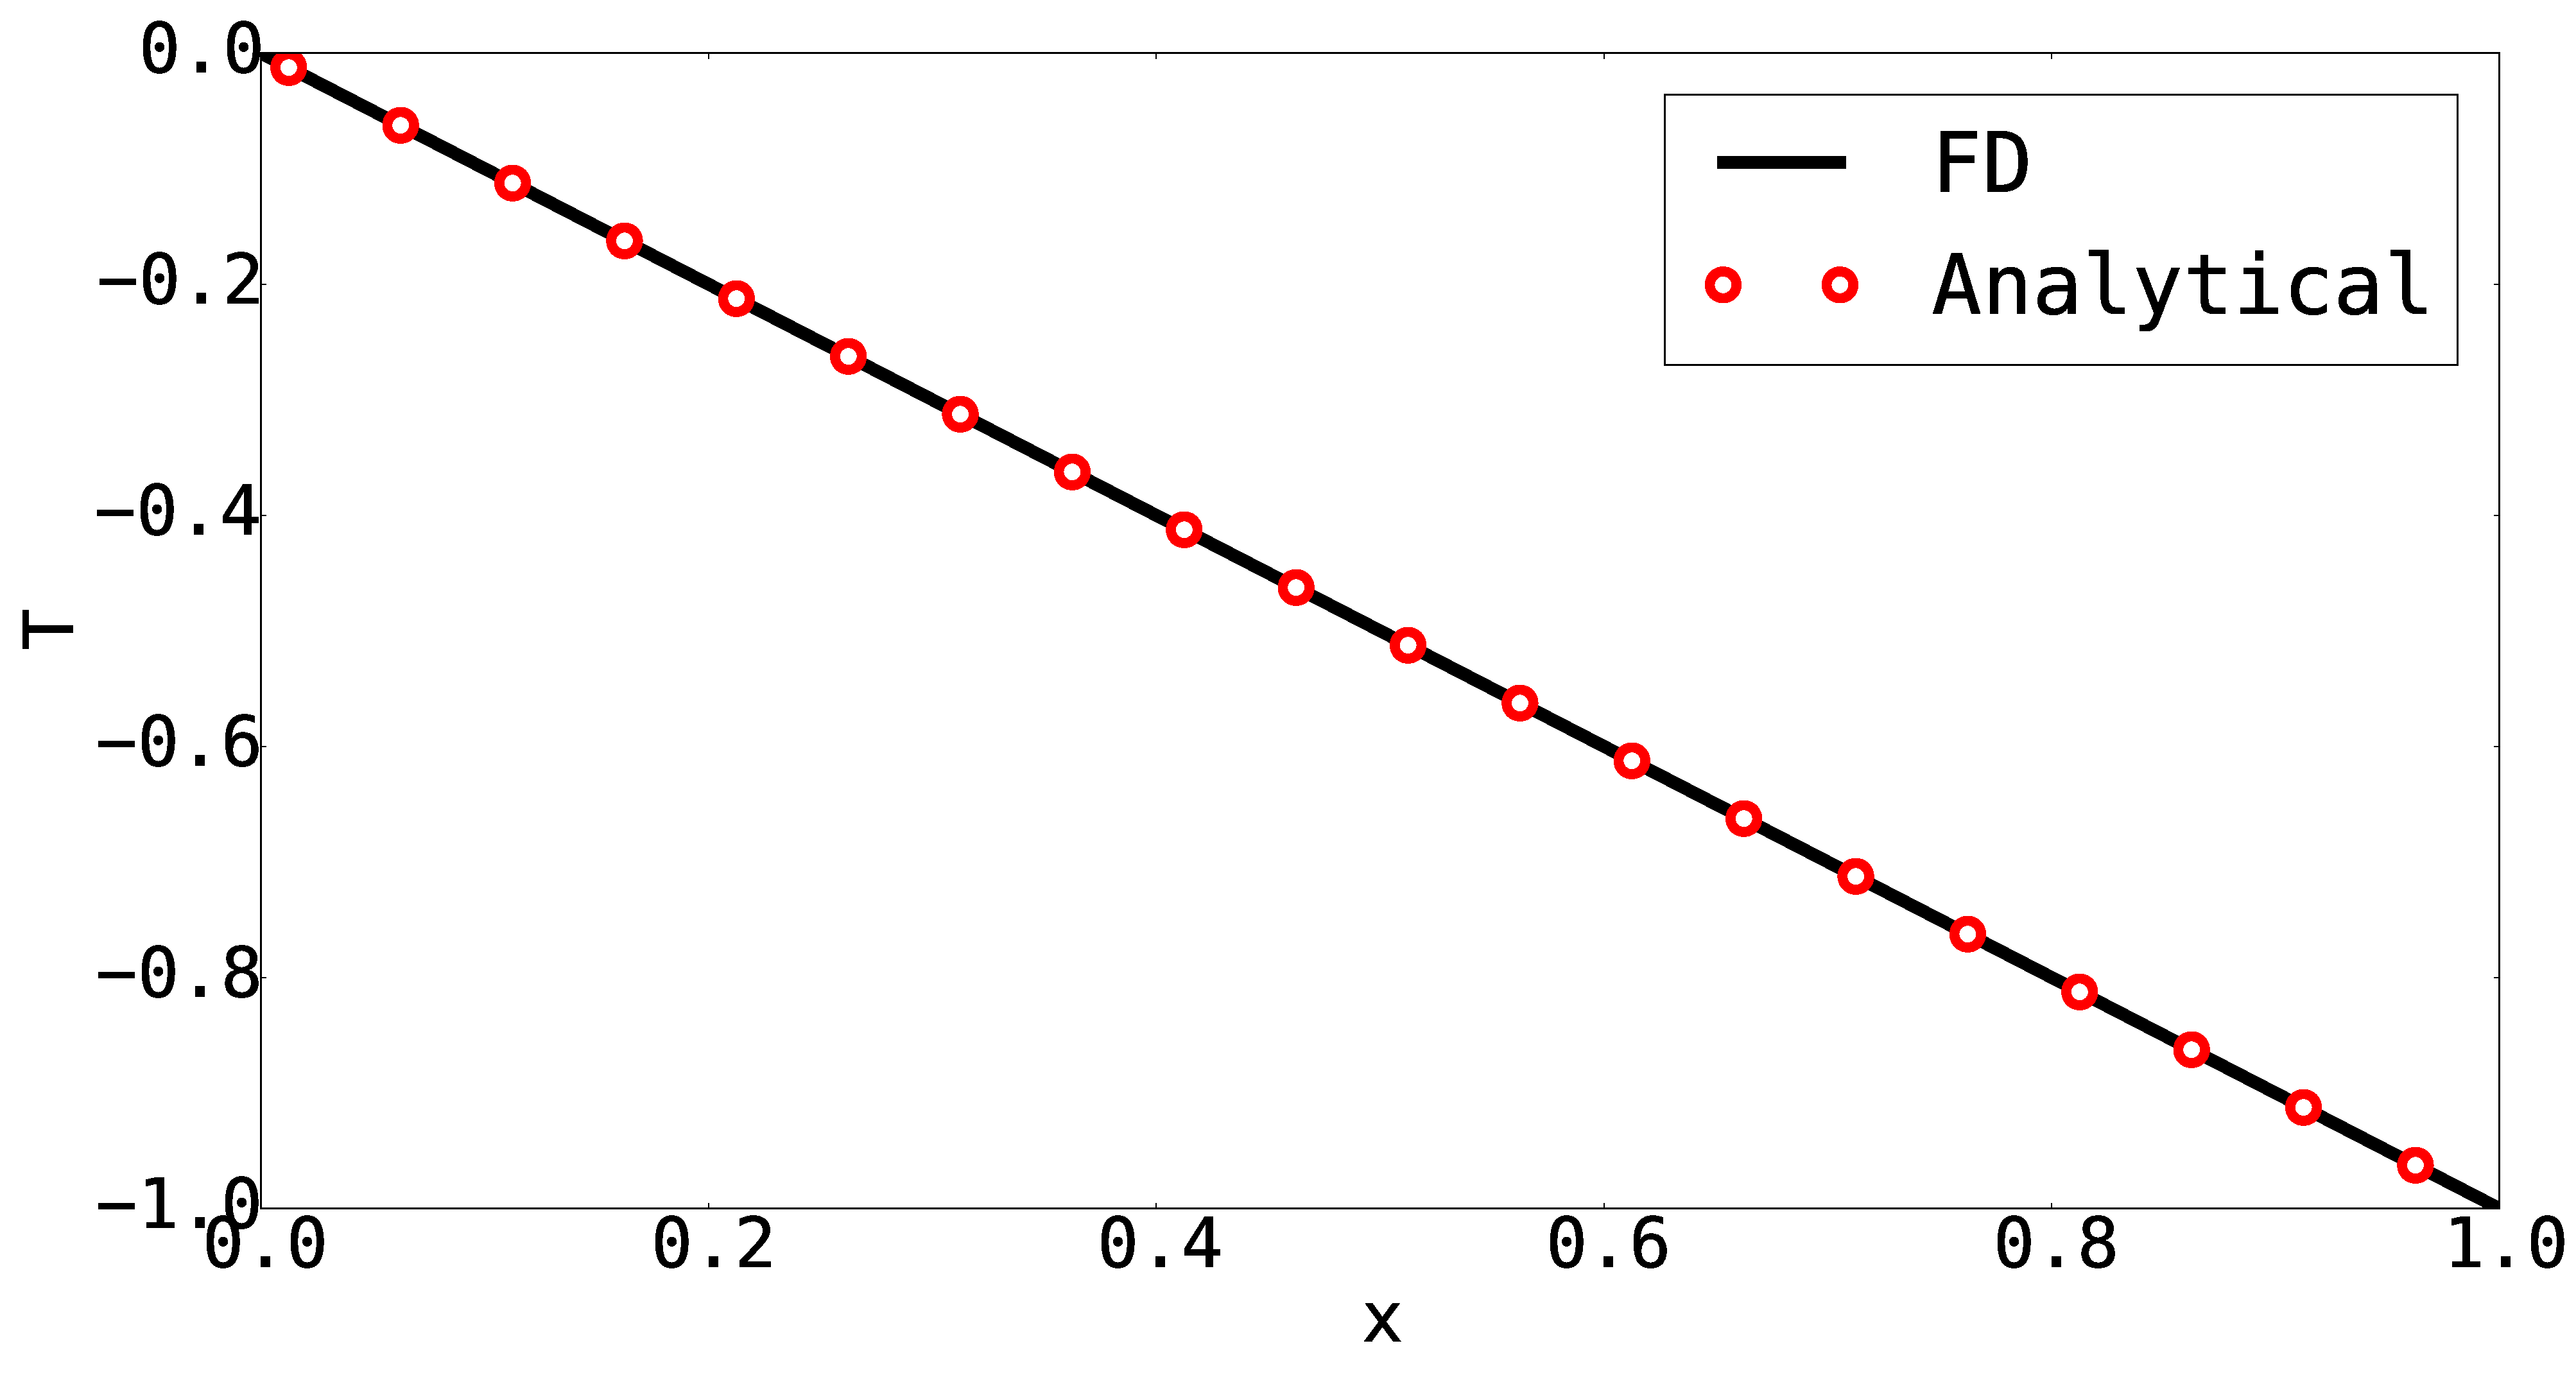
\includegraphics[width=6.5cm]{Chapter_2/figure/DSA_n81.eps}
    }
    \quad
    \subfigure[$n = 161$]
    {
    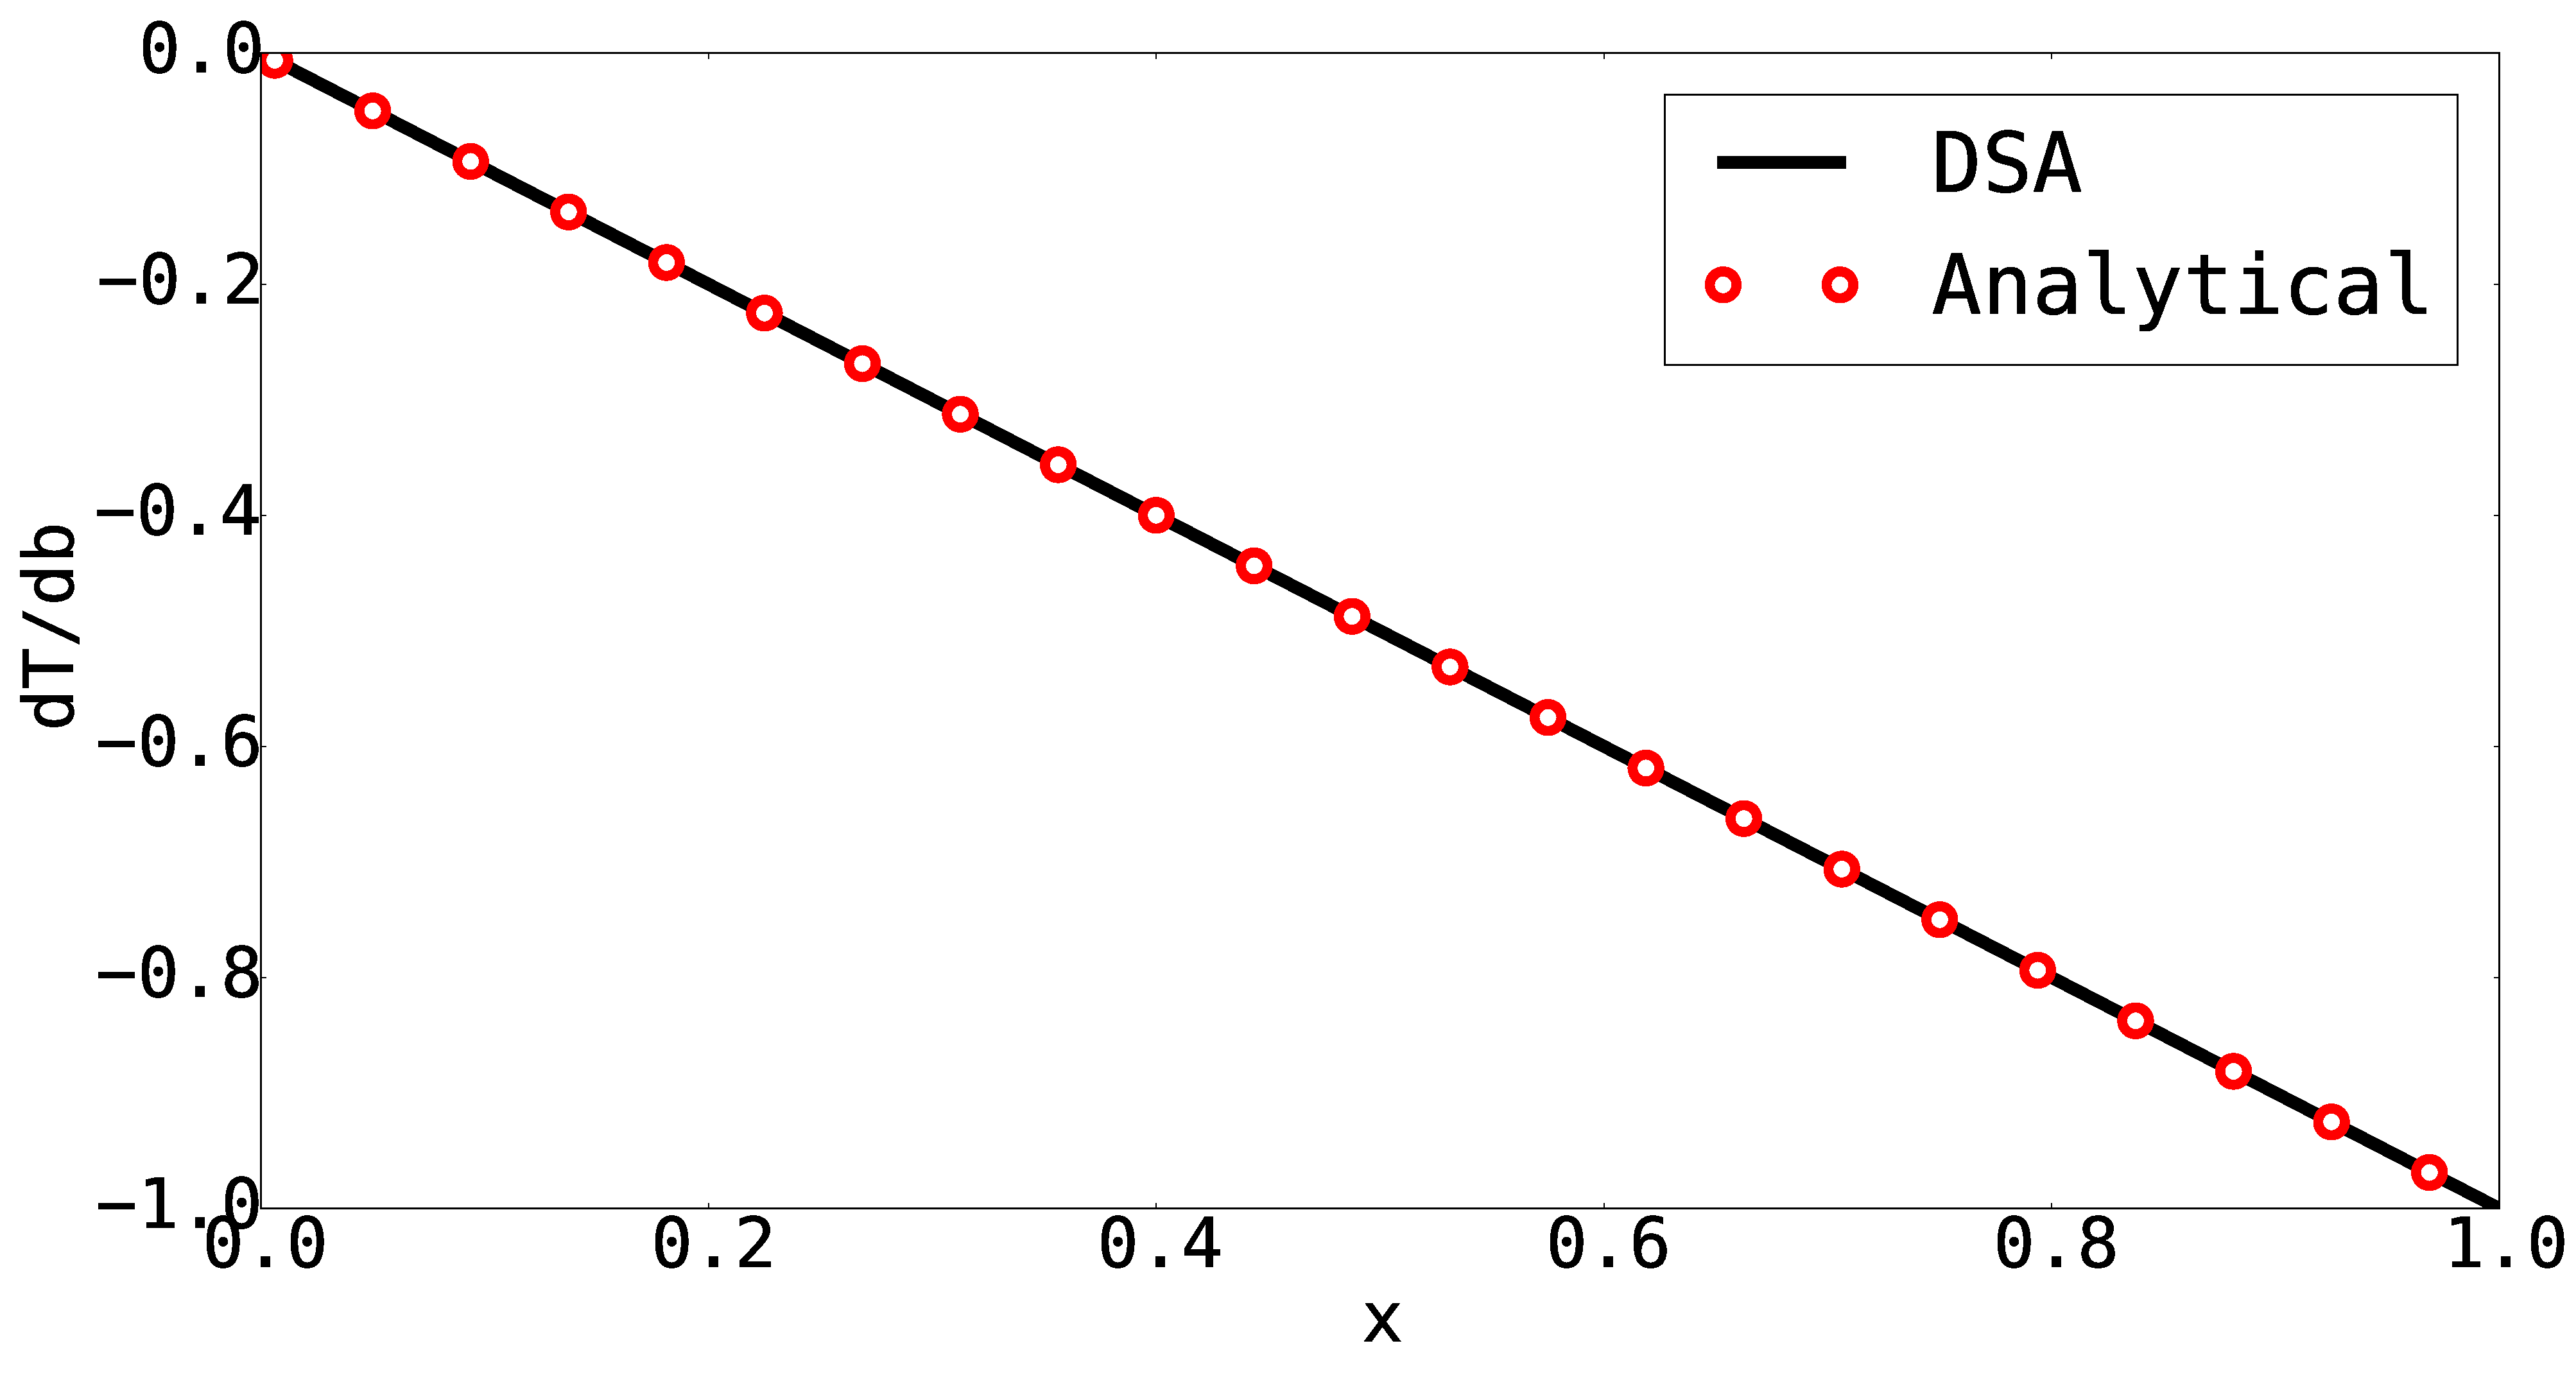
\includegraphics[width=6.5cm]{Chapter_2/figure/DSA_n161.eps}
    }
    \caption{Comparison between discrete sensitivity analysis and analytical results for different number of nodes.}
    \label{fig:C2_discreteSensitivityVerification}
\end{figure}
%
%
\begin{table}[H]
\centering
\begin{tabular}{| c | c |}
    \hline
    Number of nodes & NRMSD \\ \hline \hline
    11 & $1.68 \times 10^{-16}$ \\ \hline
    41 & $2.49 \times 10^{-15}$ \\ \hline
    81 & $1.49 \times 10^{-15}$ \\ \hline
    161 & $2.85 \times 10^{-15}$ \\ \hline
\end{tabular}
\caption{RMSE value for different number of nodes.}
\label{table:C2_DSA_NRMSD}
\end{table}
%
As shown in Figure \ref{fig:C2_discreteSensitivityVerification} and Table \ref{table:C2_DSA_NRMSD}, the accuracy of discrete sensitivity analysis is not affected by the number of nodes chosen to discretize the domain.

% -.-.-.-.-.-.-.-.-.-.-.-.-.-.-.-.-.-.-.-.-.-.-.-.-.-.-.-.-.-.-.-.-.-.-.-.-.-.-.-.-.-.-.-.-.-
\subsection{Implementation on solid mechanics problem}
Finite elements are used to discretized the axial bar problem is shown in Figure \ref{fig:C2_axialBarPhysicalShape}. The governing equation of \eqref{eq:C2_axialBarGE} is discretized using a uniform mesh, linear shape functions, and one point Gauss integration. As mentioned in Section \ref{section:C2_solid_mechanics_benchmark}, the design variable is selected as the length of the bar affecting the distances between the nodes. To keep the local and total derivatives equal, we fix the interior computational nodes in space and change the length of the bar by only moving the last node. Therefore, the shape design variable only affects the size of the last element and should be included in the discretized equations. This is shown in Figure \ref{fig:C2_axialBarComputationalDomain}. Since the internal nodes do not move, the design velocity is zero for these nodes.
%
\begin{figure}[H]
    \centering
    \subfigure[Original domain]
    {
    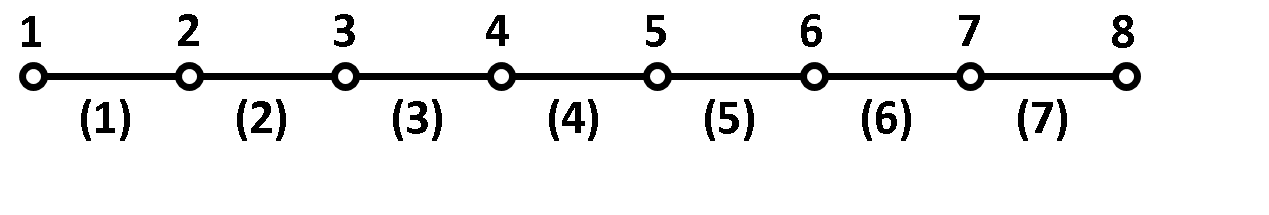
\includegraphics[width=14.0cm]{Chapter_2/figure/bar_computational_before.png}
    }
    \\
    \subfigure[Deformed domain]
    {
    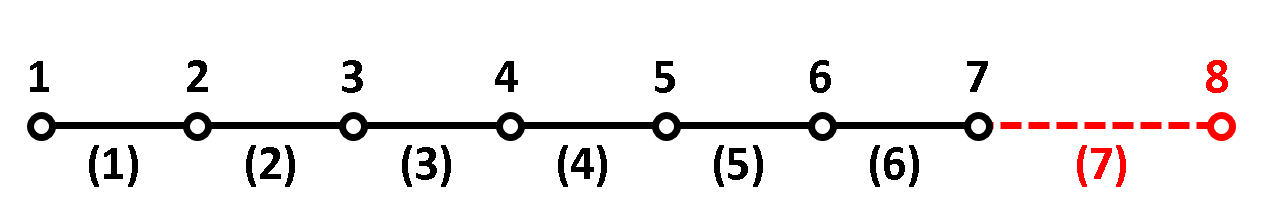
\includegraphics[width=14.0cm]{Chapter_2/figure/bar_computational_after.png}
    }
    \caption{Changing the bar length by fixing the interior computational nodes and only moving the boundary (red) node. Node numbers are represented by $i$ and element numbers by $(i)$.}
    \label{fig:C2_axialBarComputationalDomain}
\end{figure}
%
For the case of three elements, the stiffness matrix is written as
%
\begin{equation}\label{eq:C2_stiffnessMatrixOfBar}
    [K] = 
    EA
    \begin{bmatrix}
    1/l_1 & -1/l_1 & 0 & 0 \\
    -1/l_1 & 1/l_1 + 1/l_2 & -1/l_2 & 0 \\
    0 & -1/l_2 & 1/l_2 + 1/l_3 & -1/l_3 \\
    0 & 0 & -1/l_3 & 1/l_3
    \end{bmatrix}
\end{equation}
%
Where $l_i$ are the lengths of the elements. It should be noted that only $l_3$ is affected by changing the length of the domain in this formulation of the problem. The discretized equation for this problem is written as shown in Equation \eqref{eq:C2_discretizedBarEquation}.
%
\begin{equation}\label{eq:C2_discretizedBarEquation}
    [K - K_s] [U] = [F_d] - [F_p]
\end{equation}
%
Where $[K]$ is the stiffness matrix of the bar; $[K_s]$ is the stiffness of the spring boundary; $[F_d]$ is the distributed load; and $[F_p]$ is the point load. The point load is substracted because of its negative direction for this problem. For the case of $EA = 1$, $F_d = \sin(\pi x / 2)$, $L = 1$, $F_p = 1 / \pi$, and $K_s = 10$ the solution of Equation \eqref{eq:C2_discretizedBarEquation} is compared with the analytical results of the problem as shown in Equation \eqref{eq:C2_axialBarSolution} in Figure \ref{fig:C2_axialBarSolution}. We chose Normalized Root-Mean-Square Error (NRMSE) as the metric of comparison. This is calculated as shown in Equation \eqref{eq:C2_NRMSE_beam}
%
\begin{equation}\label{eq:C2_NRMSE_beam}
    NRMSE = \dfrac{\sqrt{\dfrac{\sum_{t=1}^n \left( \hat{y}_t - y \right)^2}{n}}}{y_{max} - y_{min}}
\end{equation}
%
where $\hat{y}_t$ is numerical and $y$ is the analytical result.
%
\begin{figure}[h]
    \centering
    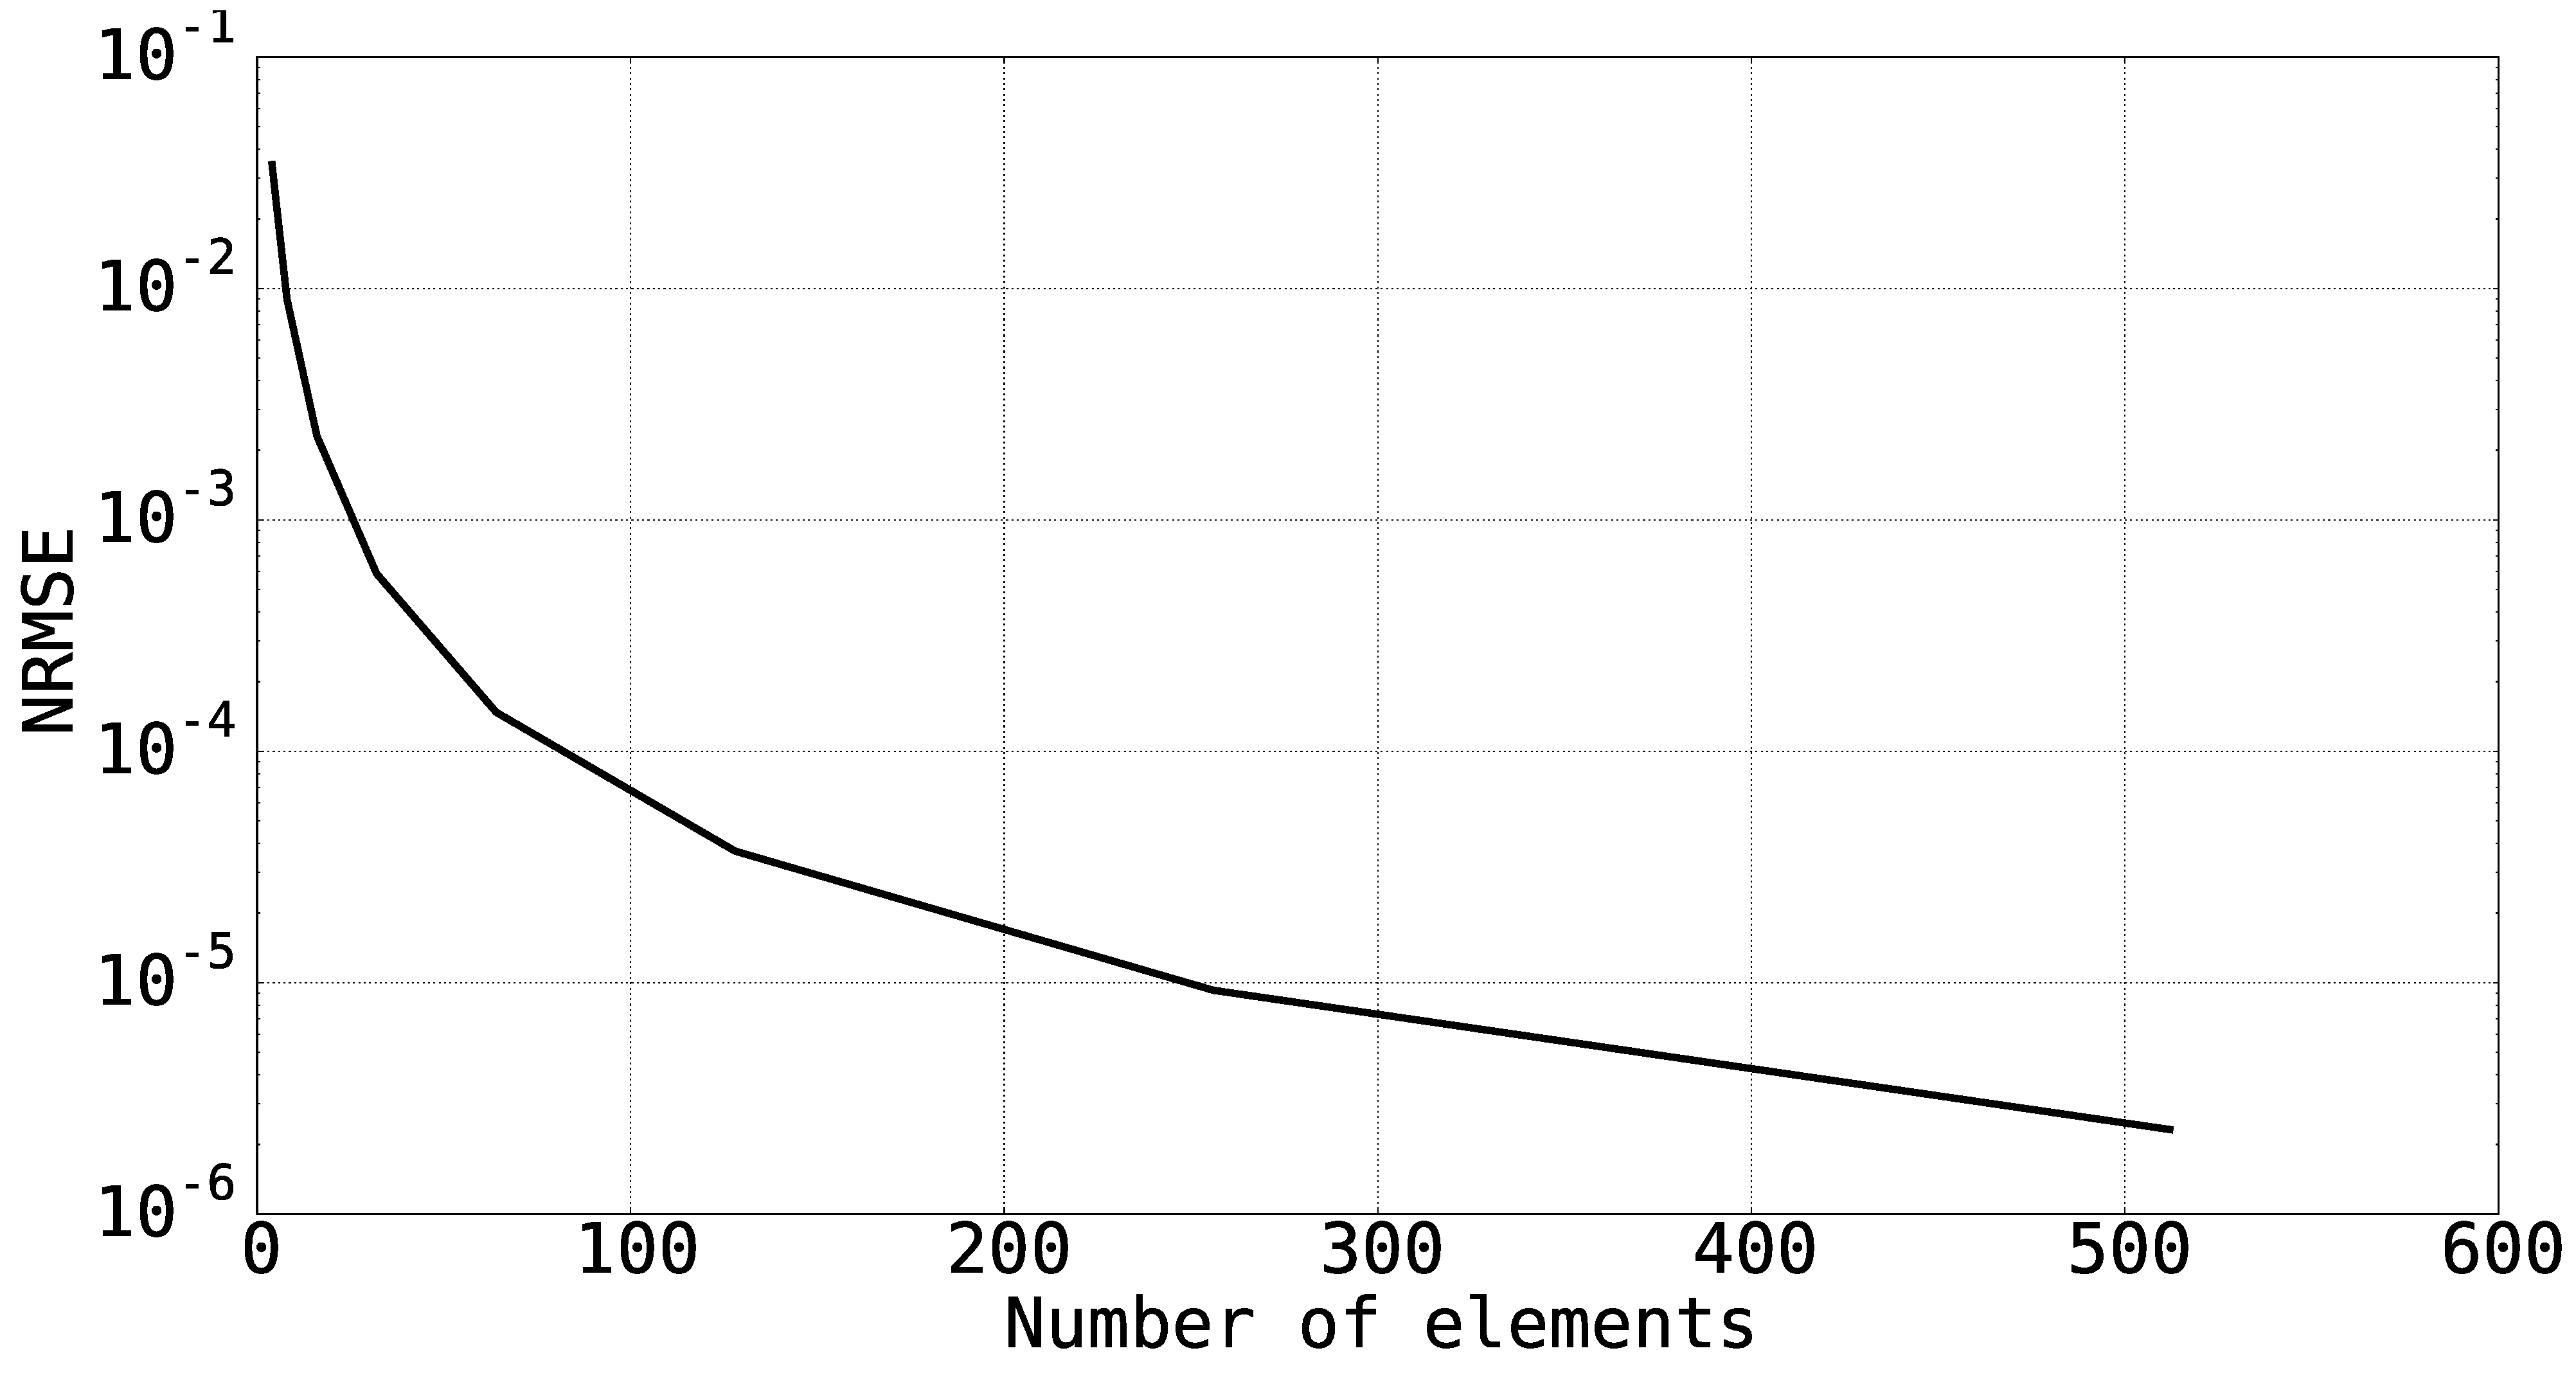
\includegraphics[width=14.00cm]{Chapter_2/figure/axial_bar_governing_equation_mesh_convergence.eps}
    \caption{Mesh convergence of the finite elements analysis for axial bar.}
    \label{fig:C2_axialBarSolution}
\end{figure}
%
The discrete sensitivity equation is derived by differentiating Equation \eqref{eq:C2_discretizedBarEquation} with respect to the shape of the domain as shown in Equation \eqref{eq:C2_discretizedSAequation_beforeSimplification}.
%
\begin{equation}\label{eq:C2_discretizedSAequation_beforeSimplification}
    \left[ \frac{\partial K}{\partial b} - \frac{\partial K_s}{\partial b} \right] [U] + 
    [K - K_s] \left[ \frac{\partial U}{\partial b} \right] = 
    \left[ \frac{\partial F_d}{\partial b} \right] - 
    \left[ \frac{\partial F_p}{\partial b} \right]
\end{equation}
%
Where $b$ is the design variable. $[K_s]$ is not affected by the design variable; therefore, its derivative with respect to $b$ is equal to zero. The same argument can be made for the point load $F_p$. Using these observations, Equation \eqref{eq:C2_discretizedSAequation_beforeSimplification} is simplified as:
%
\begin{equation}\label{eq:C2_discretizedSensitivityEquation}
    \left[ \frac{\partial U}{\partial b} \right] = 
    [K - K_s]^{-1}
    \left\{
    \left[ \frac{\partial F_d}{\partial b} \right] - \left[ \frac{\partial K}{\partial b} \right] [U]
    \right\}
\end{equation}
%
In Equation \eqref{eq:C2_discretizedSensitivityEquation}, $[U]$ is known as the result of solving the governing equation \eqref{eq:C2_discretizedBarEquation} and $\dfrac{\partial F_d}{\partial b}$ is easily calculated since the distributed force is analytically known. $\dfrac{\partial K}{\partial b}$ is calculated by differentiating Equation \eqref{eq:C2_stiffnessMatrixOfBar}. It should be noted that the change in bar length, $L$, only affects $l_3$. Therefore, $\dfrac{\partial l_3}{\partial L}$ is equal to one. Finally, the sensitivity of the stiffness matrix to the shape design variable for a simple case of Equation \eqref{eq:C2_stiffnessMatrixOfBar} is written as:
%
\begin{equation}\label{eq:C2_sensitivityOfStiffnessMatrixOfBar}
    \left[ \frac{\partial K}{\partial L} \right] = 
    -EA
    \begin{bmatrix}
    0 & 0 & 0 & 0 \\
    0 & 0 & 0 & 0 \\
    0 & 0 & 1/l_3^2 & -1/l_3^2 \\
    0 & 0 & -1/l_3^2 & 1/l_3^2
    \end{bmatrix}
\end{equation}
%
The sensitivity results of solving the discrete Equation \eqref{eq:C2_discretizedSensitivityEquation} are compared with the analytical result from Equation \eqref{eq:C2_axialBarSensitivitySolution}. This comparison is shown as NRMSE values in Figure \ref{fig:C2_barDiscreteSensitivityAnalysis}. As shown here, the analytical and discrete sensitivity results agree very well. Moreover, the error decreases as we increase the number of elements.
%
\begin{figure}[h]
    \centering
    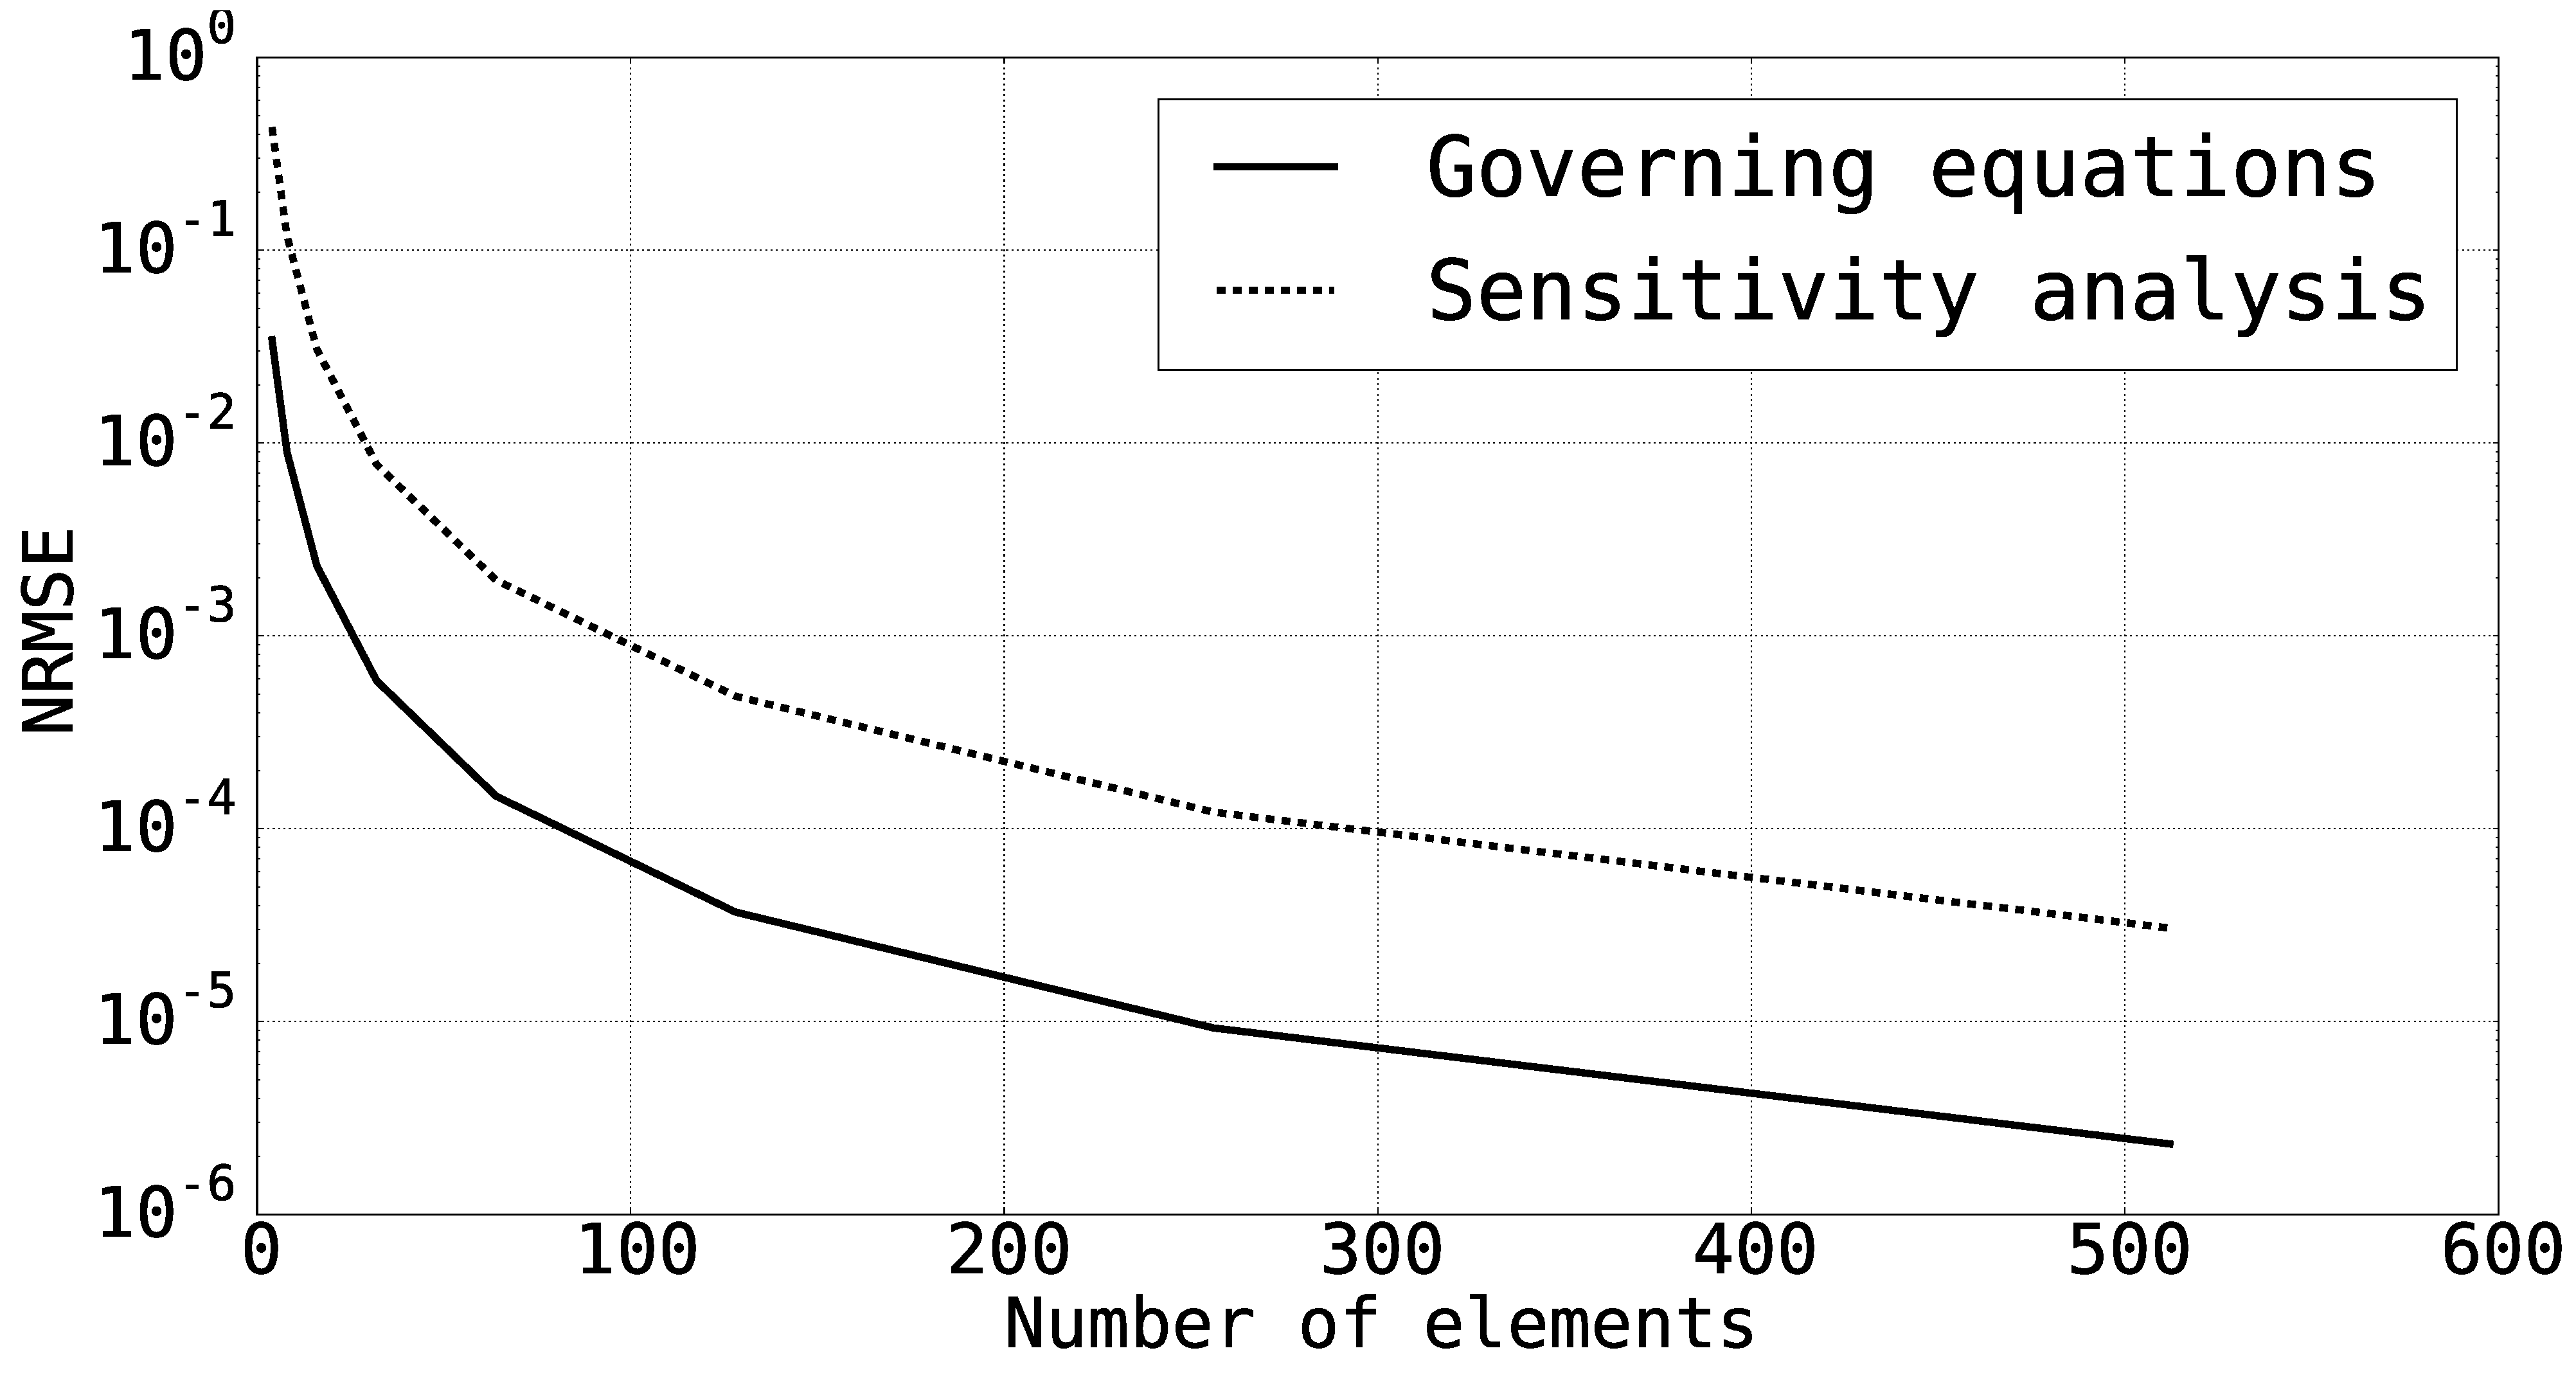
\includegraphics[width=14.00cm]{Chapter_2/figure/axial_bar_discrete_sensitivity_analysis.eps}
    \caption{Mesh convergence of the discrete sensitivity analysis for the axial bar.}
    \label{fig:C2_barDiscreteSensitivityAnalysis}
\end{figure}
%